\documentclass[11pt,a4paper]{article}

\usepackage[margin=2.2cm]{geometry}
\usepackage{lmodern}
\usepackage[T1]{fontenc}
\usepackage{microtype}
\usepackage{amsmath,amssymb}
\usepackage{graphicx}
\usepackage{booktabs}
\usepackage{tabularx}
\usepackage{longtable}
\usepackage{float}
\usepackage{caption}
\usepackage{subcaption}
\usepackage{enumitem}
\usepackage{xcolor}
\usepackage{listings}
\usepackage{fancyhdr}
\usepackage[hidelinks]{hyperref}

\graphicspath{{img/}{../evidence/}{../output/figures/}}

\definecolor{codebg}{HTML}{F4F4F2}
\lstset{basicstyle=\ttfamily\small, backgroundcolor=\color{codebg}, breaklines=true,
        frame=none, columns=fullflexible, keepspaces=true, xleftmargin=0.5em, aboveskip=0.6em, belowskip=0.6em}
\captionsetup{font=small, labelfont=bf}
\setlist{itemsep=0.2em, topsep=0.3em}
\setlength{\parskip}{0.45em}
\setlength{\parindent}{0pt}
\setlength{\emergencystretch}{3em}  % let long \texttt names wrap instead of overflowing
\DeclareRobustCommand{\_}{\textunderscore\allowbreak}  % allow line breaks after underscores in names

\newcommand{\ct}[1]{\texttt{#1}}
\makeatletter
\newcommand\rawinput[1]{\@@input #1 }
\makeatother

\newcommand{\csdir}{Client $\rightarrow$ Server}
\newcommand{\scdir}{Server $\rightarrow$ Client}

\pagestyle{fancy}
\fancyhf{}
\lhead{\small Information Security -- Assignment 01}
\rhead{\small 23i-0688}
\cfoot{\small \thepage}

\begin{document}

% ------------------------------------------------------------------ title page
\begin{titlepage}
\centering
\vspace*{3.5cm}
{\Large Information Security\par}
{\large Assignment 01 \,--\, Fall 2026\par}
\vspace{1.8cm}
{\huge\bfseries Breaking PsycoSupport\par}
\vspace{0.4cm}
{\Large Al-Kindi Frequency Analysis of an Affine-Cipher\\Client--Server Channel\par}
\vspace{2.5cm}
{\large Syed Muhammad Faateh Haneef\par}
{\large 23i-0688\par}
\vfill
{\large 22 October 2026\par}
\end{titlepage}

\tableofcontents
\newpage

% ------------------------------------------------------------------ summary
\section*{Summary}
\addcontentsline{toc}{section}{Summary}

The PsycoSupport client and server were deployed fully offline on Linux, five patient sessions were sent, and
all traffic on the loopback interface was captured. This produced \textbf{10 ciphertexts} (5 in each direction).
Using Al-Kindi frequency analysis, every affine key was recovered from the ciphertext alone and \textbf{all 10
ciphertexts were decrypted}.

\begin{table}[H]\centering
\caption{Recovered keys. The same key is used in both directions for a given mood.}
\begin{tabular}{c c c c l}
\toprule
Mood & $(a,b)$ & $a^{-1} \bmod 26$ & Sessions & Decryption rule \\
\midrule
2  & (5, 4)   & 21 & 2    & $D(y)=21(y-4) \bmod 26$ \\
5  & (11, 10) & 19 & 1, 3 & $D(y)=19(y-10) \bmod 26$ \\
8  & (17, 16) & 23 & 4    & $D(y)=23(y-16) \bmod 26$ \\
10 & (21, 20) & 5  & 5    & $D(y)=5(y-20) \bmod 26$ \\
\bottomrule
\end{tabular}
\end{table}

Main findings:
\begin{itemize}
\item The key depends only on the \textbf{mood}: $a = 2m+1$, $b = 2m \pmod{26}$. The mood is sent \emph{unencrypted},
      so the key is effectively public.
\item \scdir{} is a plain affine cipher on upper-case letters. \csdir{} first writes every character as two hex digits and
      then affine-encrypts the digits, so one character becomes two cipher letters.
\item Every reply starts with the username (\ct{FAATEH \ldots}), which is a free known-plaintext crib.
\item Using only the recovered protocol, the server was rebuilt as an Ollama-backed \ct{server.py}. The original
      client works with it, including at a mood that was never captured (Section~\ref{sec:ownserver}).
\item The two recommended fixes (TLS~1.3 and UNIX domain sockets) were \textbf{implemented and tested}
      (Section~\ref{sec:fixes}). The same attack fails against them.
\end{itemize}

% ================================================================== 1
\section{Ciphertext Collection \& Evidence}

\subsection{Offline lab environment}
All work ran on one machine inside an isolated Linux environment (Ubuntu 24.04 under WSL2, NVIDIA RTX 3050 Ti).
The provided \ct{client} and \ct{server} programs are Linux executables, so they were run there.

\begin{enumerate}
\item \textbf{Ollama installation.} Installed with the official script. The URL in the handout is missing the script
      path; the working command is:
\begin{lstlisting}
curl -fsSL https://ollama.com/install.sh | sh      # Ollama 0.40.4, service on 127.0.0.1:11434
\end{lstlisting}
\item \textbf{Model provisioning.} \ct{ollama pull llama3.2} (3B parameters, 2.0\,GB), tested with a one-line prompt
      (Figure~\ref{fig:setup}).
\item \textbf{Server binding.} The supplied \ct{server} calls Groq's cloud API with the model
      \ct{llama-3.1-8b-instant}, which Groq has since retired, so every request failed with HTTP 404. The handout says the server's
      functionality must not change, so the executable was left untouched. Instead, the Groq client library inside it
      was pointed at a small local relay (\ct{relay.py}, submitted) through its standard \ct{GROQ\_BASE\_URL} setting.
      The relay swaps the model name for \ct{llama3.2} and forwards the request to Ollama:
\begin{lstlisting}
client --(9999, encrypted)--> server --(8000)--> relay.py --(11434)--> Ollama llama3.2

python3 relay.py                                        # tab 1
GROQ_BASE_URL=http://127.0.0.1:8000 ./server            # tab 2: "[SERVER] Listening on 0.0.0.0:9999"
./client                                                # tab 3: IP 127.0.0.1, port 9999, user Faateh
\end{lstlisting}
\end{enumerate}

The server listens on TCP port \textbf{9999} (not 5000 as suggested in the handout). The API-key field is ignored,
as instructed; the dummy value \ct{dummy} was typed.

All ciphertexts in this report were captured from this original, unmodified server, so the analysis attacks the
real application. No server source was provided, so its protocol had to be recovered first. Once it was
(Sections~2--3), the server was re-implemented as a standalone Ollama-backed \ct{server.py} and validated against
the original client (Section~\ref{sec:ownserver}).

\begin{figure}[H]\centering
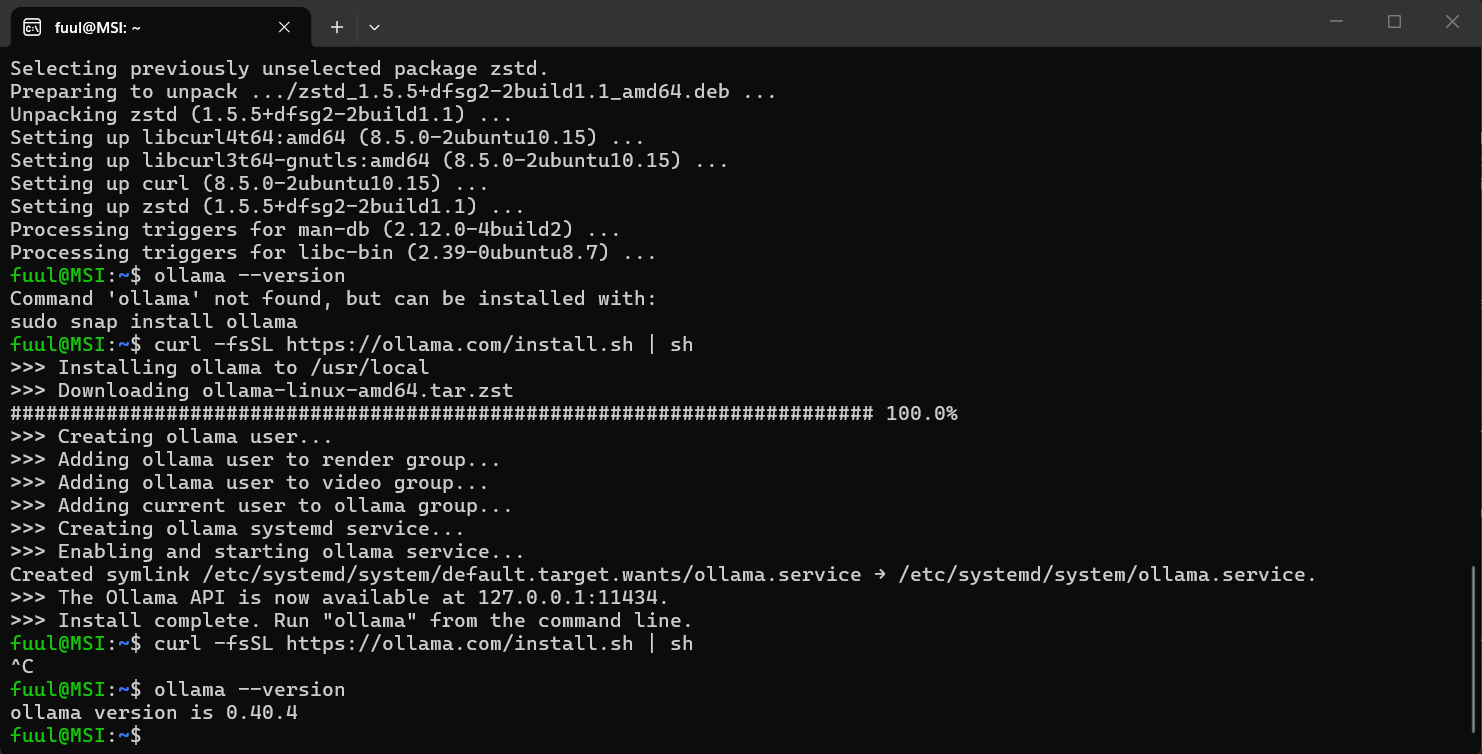
\includegraphics[width=0.62\linewidth]{01_ollama_install_terminal.png}\\[0.4em]
\begin{subfigure}{0.49\linewidth}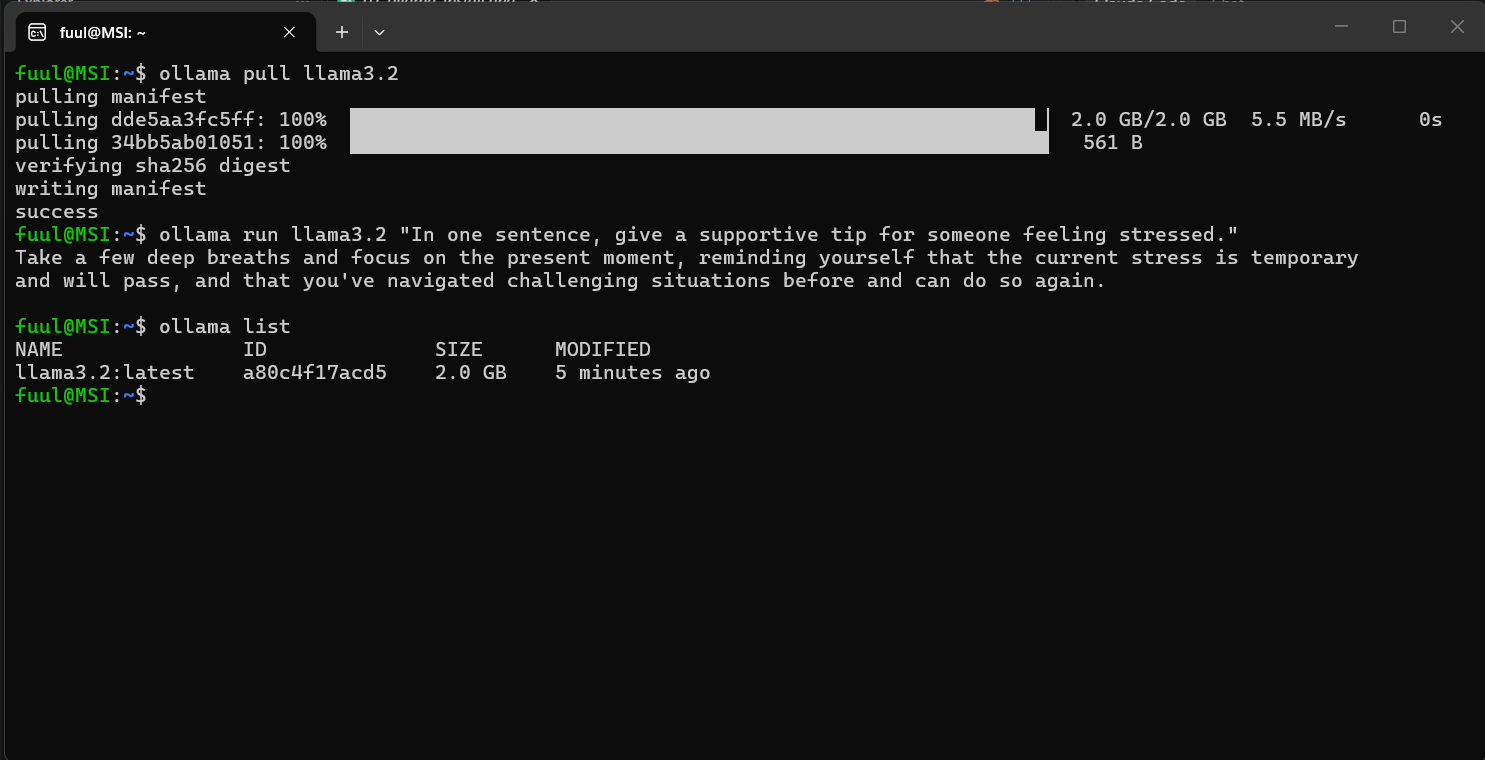
\includegraphics[width=\linewidth]{02_model_pull_test.png}
\caption{Model downloaded and answering locally.}\end{subfigure}\hfill
\begin{subfigure}{0.49\linewidth}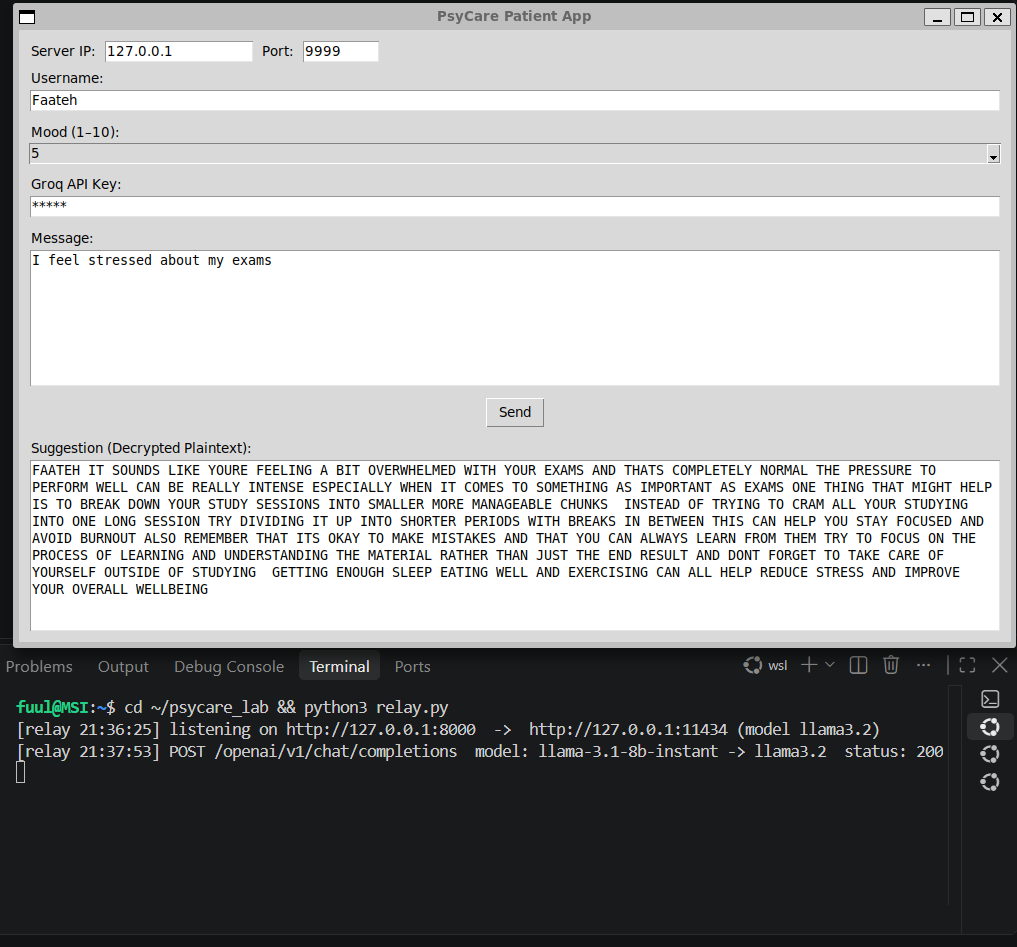
\includegraphics[width=\linewidth]{03_first_run.png}
\caption{First end-to-end run; the relay logs \ct{status: 200}.}\end{subfigure}
\caption{Offline pipeline working. Top: Ollama installed (\ct{ollama version is 0.40.4}).}
\label{fig:setup}
\end{figure}

\subsection{Capture method}
Traffic was captured on the loopback interface, filtered to the application port:
\begin{lstlisting}
sudo tcpdump -i lo -w ~/psycare_lab/capture.pcap 'tcp port 9999'
\end{lstlisting}
The filter deliberately leaves out the server-to-relay hop (port 8000), so the capture contains only what an
eavesdropper on the client--server channel sees. \textbf{50 packets} were captured across \textbf{5 TCP
conversations}, one per session. Ciphertexts were extracted from the \ct{.pcap} by
a small Python script that reassembles each TCP stream, and cross-checked with Wireshark's \emph{Follow TCP Stream}
(Figure~\ref{fig:wireshark}).

\subsection{Test cases}
The username was always \ct{Faateh}, as instructed. Moods were varied so the effect of the mood could be studied, and
two sessions share mood~5 so they could be compared.

\begin{table}[H]\centering
\caption{The five test sessions (concerns are synthetic).}
\begin{tabularx}{\textwidth}{c c c X}
\toprule
Session & Mood & Ciphertexts & Concern typed into the client \\
\midrule
1 & 5  & C1, S1 & I have not been sleeping well and I feel tired all the time \\
2 & 2  & C2, S2 & I feel stressed about my exams \\
3 & 5  & C3, S3 & My friends have been ignoring me lately and I feel lonely \\
4 & 8  & C4, S4 & I got a good grade but I still worry about the next semester \\
5 & 10 & C5, S5 & I feel great today and want tips to keep my motivation up \\
\bottomrule
\end{tabularx}
\end{table}

\subsection{Message format on the wire}
Each conversation is one JSON request followed by one JSON reply (session~1 shown, values shortened):
\begin{lstlisting}
C->S {"username_enc": "CYYVYVJCYNYU", "mood": 5, "message_enc": "CFGKYUYVJYYNGKYI...", "api_key_enc": "YCJNYXYXJF"}
S->C {"ciphertext": "NKKLCJ UL AIWXRA BUQC OIWPC YIUXY LJPIWYJ K LIWYJ ..."}
\end{lstlisting}
Three things are visible before any cryptanalysis:
\begin{itemize}
\item the \ct{mood} is sent in \textbf{plaintext};
\item \csdir{} fields are twice as long as their plaintext (\ct{Faateh}, 6 characters $\rightarrow$ 12 letters);
\item \scdir{} keeps spaces, so word lengths leak.
\end{itemize}

\subsection{Ciphertext inventory}
All ten ciphertexts are listed in full in \ct{ciphertexts.csv}.

\begin{table}[H]\centering\small
\caption{Captured ciphertexts (first 40 characters).}
\begin{tabular}{c l c r l}
\toprule
ID & Direction & Mood & Length & Ciphertext \\
\midrule
C1 & \csdir & 5  & 119  & \ct{CFGKYUYVJYYNGKYIYTJCGKYGYNYNYIGKJRYMYNYN}\ldots \\
C2 & \csdir & 2  & 60   & \ct{YXOEIIIDIDIMOENTNYNOIDNTNTIDIYOEIJIOIBND}\ldots \\
C3 & \csdir & 5  & 115  & \ct{CXJFGKYYJGYFYNYIYCJRGKYUYVJYYNGKYGYNYNYI}\ldots \\
C4 & \csdir & 8  & 121  & \ct{GNYQOFOLFGYQOHYQOFOLOLOGYQOFFYOHOGOXYQOY}\ldots \\
C5 & \csdir & 10 & 115  & \ct{ABKUQQQVQVQMKUQLLKQVQPLAKULAQXQAQPLBKUQP}\ldots \\
S1 & \scdir & 5  & 955  & \ct{NKKLCJ UL AIWXRA BUQC OIWPC YIUXY LJPIWYJ}\ldots \\
S2 & \scdir & 2  & 760  & \ct{DEEVYN S OER QYRQY VNEV UWALY DYYHSRI WFY}\ldots \\
S3 & \scdir & 5  & 1057 & \ct{NKKLCJ UL AIWXRA BUQC OIWPC NCCBUXY K VUL}\ldots \\
S4 & \scdir & 8  & 807  & \ct{XQQBGF WB KUSDPK VWEG IUSTG XGGVWDO Q HWB}\ldots \\
S5 & \scdir & 10 & 809  & \ct{VUUDAL GD ICYHFI RGWA ECYNA VAARGHQ GHKNAF}\ldots \\
\bottomrule
\end{tabular}
\end{table}

S1 and S3 (both mood~5) begin with the \emph{same} 27 characters, while every other mood looks different. This was the
first evidence that the key depends on the mood.

\subsection{Capture evidence}
\begin{figure}[H]\centering
\begin{subfigure}{0.49\linewidth}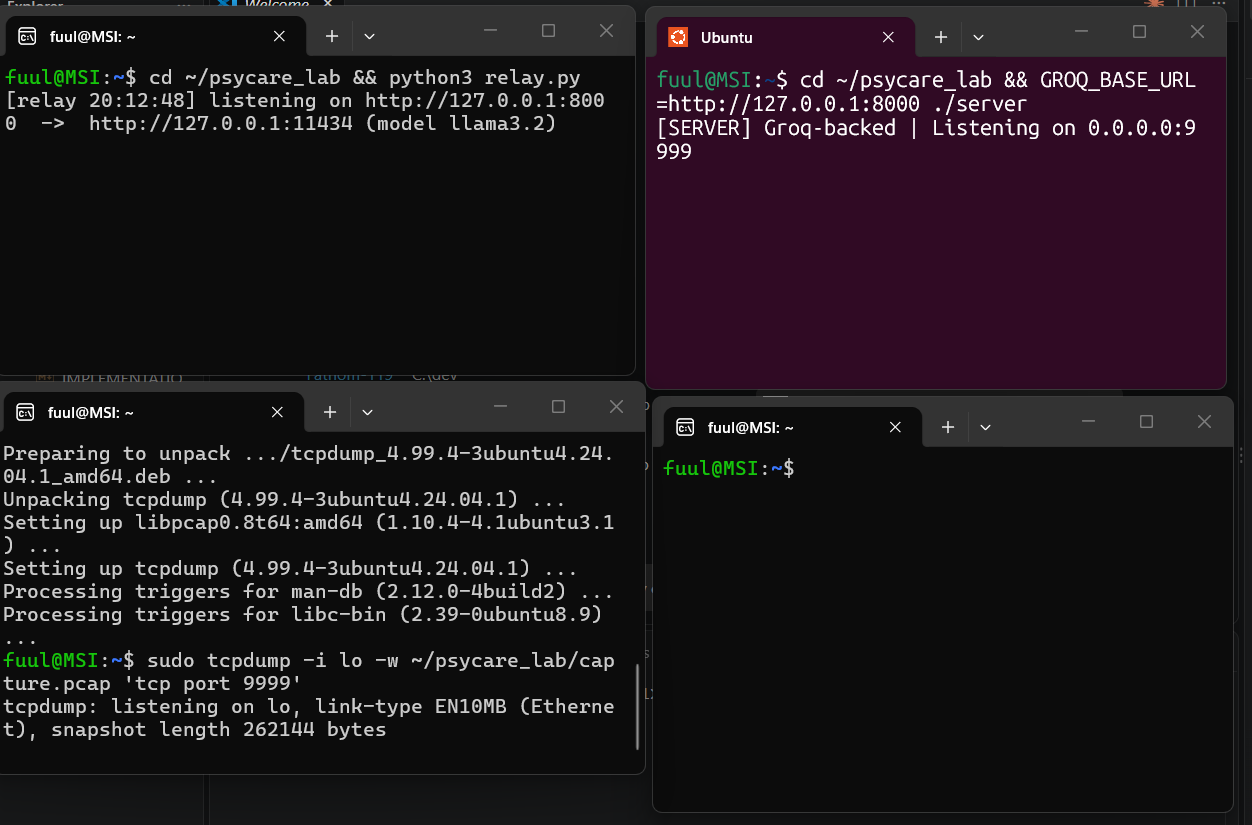
\includegraphics[width=\linewidth]{04_tcpdump_start.png}
\caption{Relay, server and \ct{tcpdump} running before the sessions.}\end{subfigure}\hfill
\begin{subfigure}{0.49\linewidth}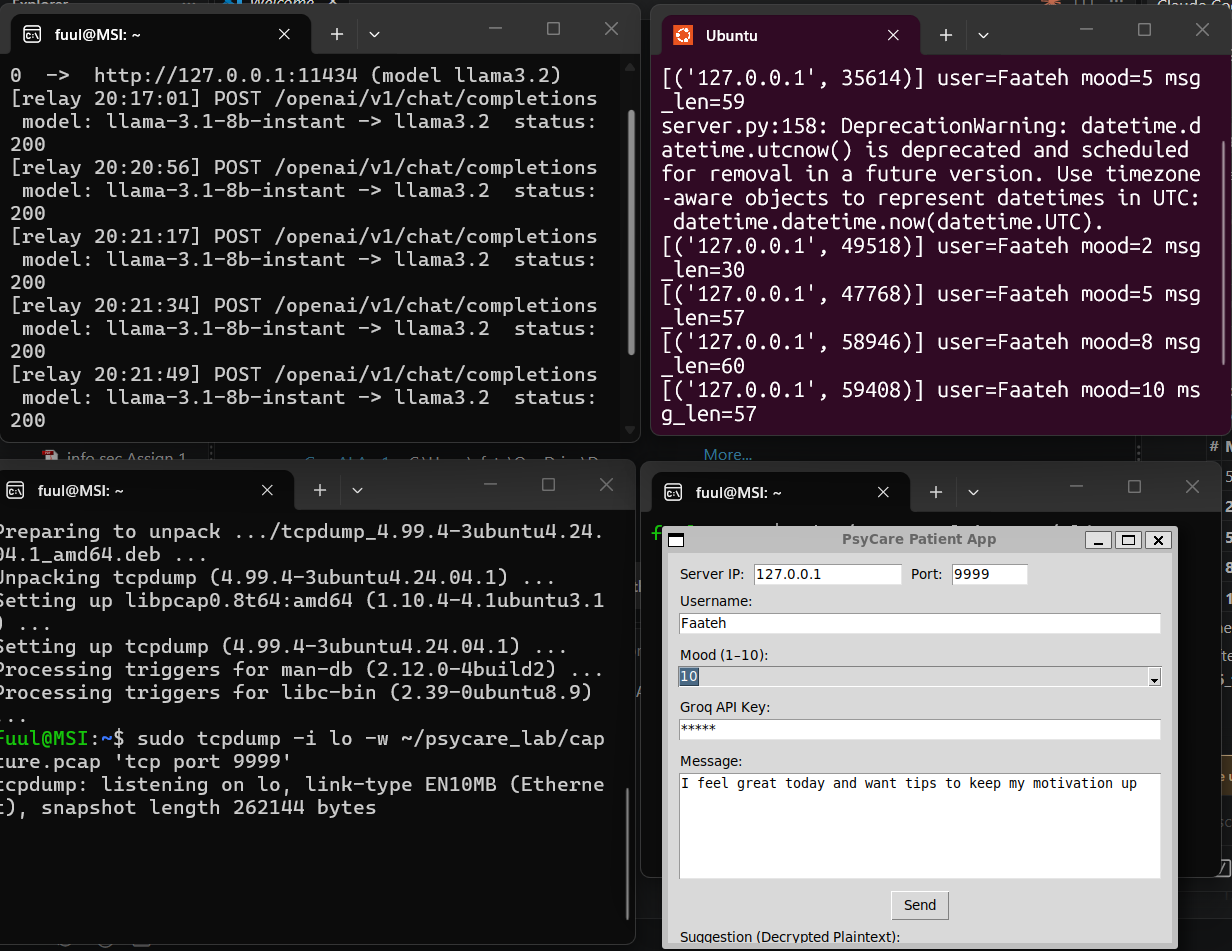
\includegraphics[width=\linewidth]{05_all_sessions.png}
\caption{All five sessions: server log shows moods 5, 2, 5, 8, 10.}\end{subfigure}\\[0.4em]
\begin{subfigure}{0.49\linewidth}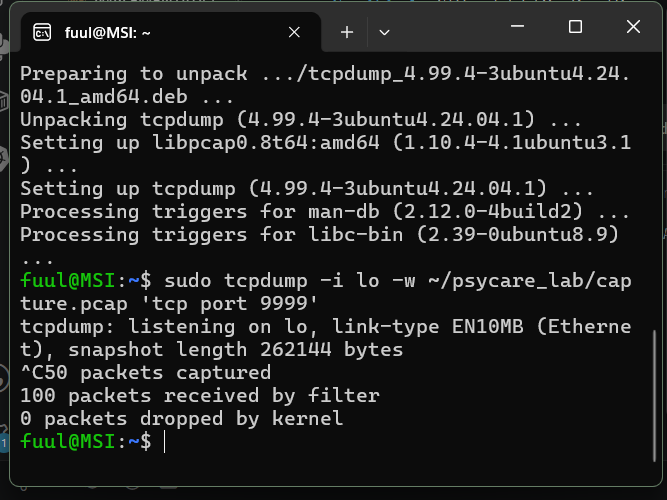
\includegraphics[width=\linewidth]{06_tcpdump_stop.png}
\caption{Capture stopped: 50 packets captured, 0 dropped.}\end{subfigure}
\caption{Capture of the five sessions on the loopback interface.}
\end{figure}

\begin{figure}[H]\centering
\begin{subfigure}{0.49\linewidth}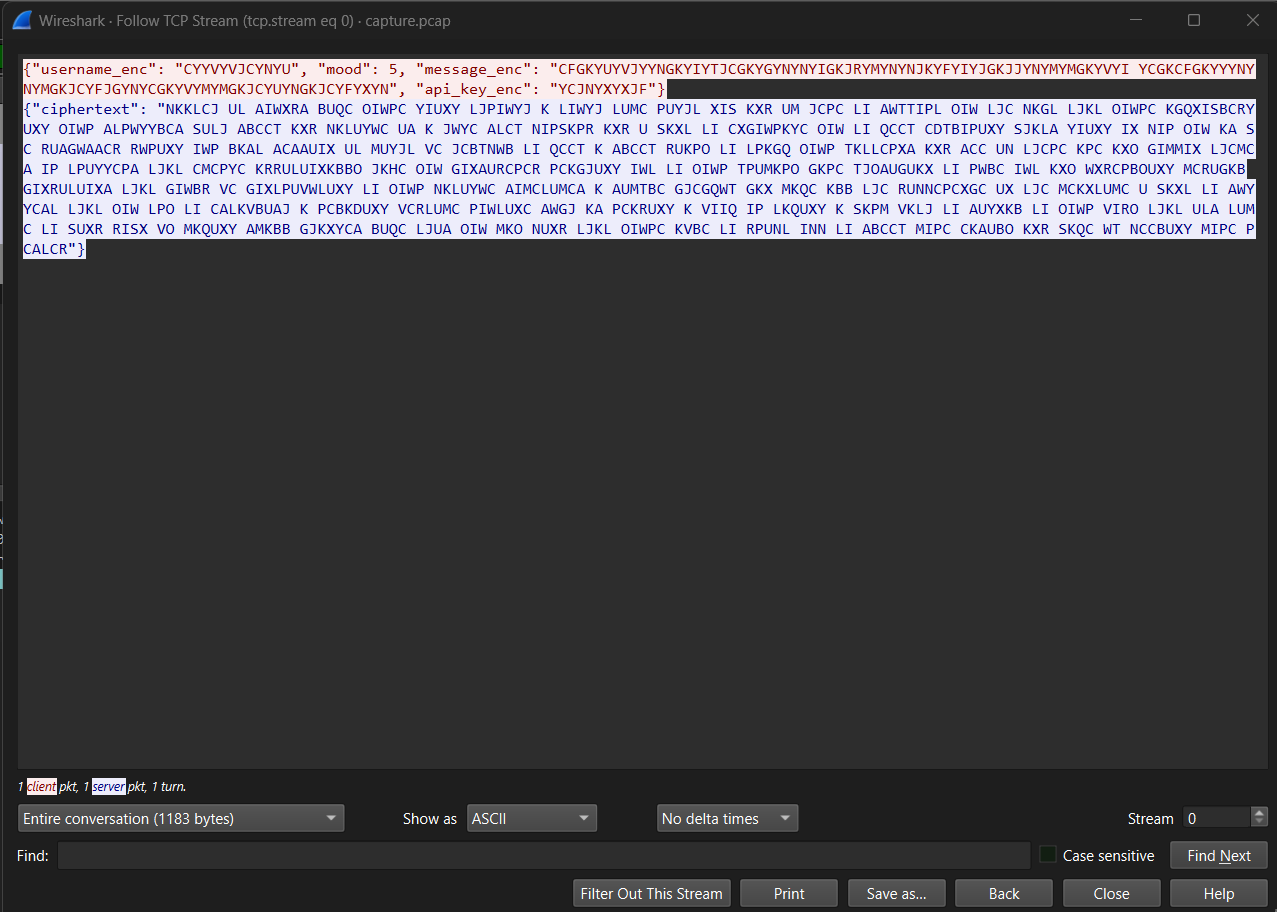
\includegraphics[width=\linewidth]{07_wireshark_stream0.png}
\caption{Stream 0: session 1, mood 5.}\end{subfigure}\hfill
\begin{subfigure}{0.49\linewidth}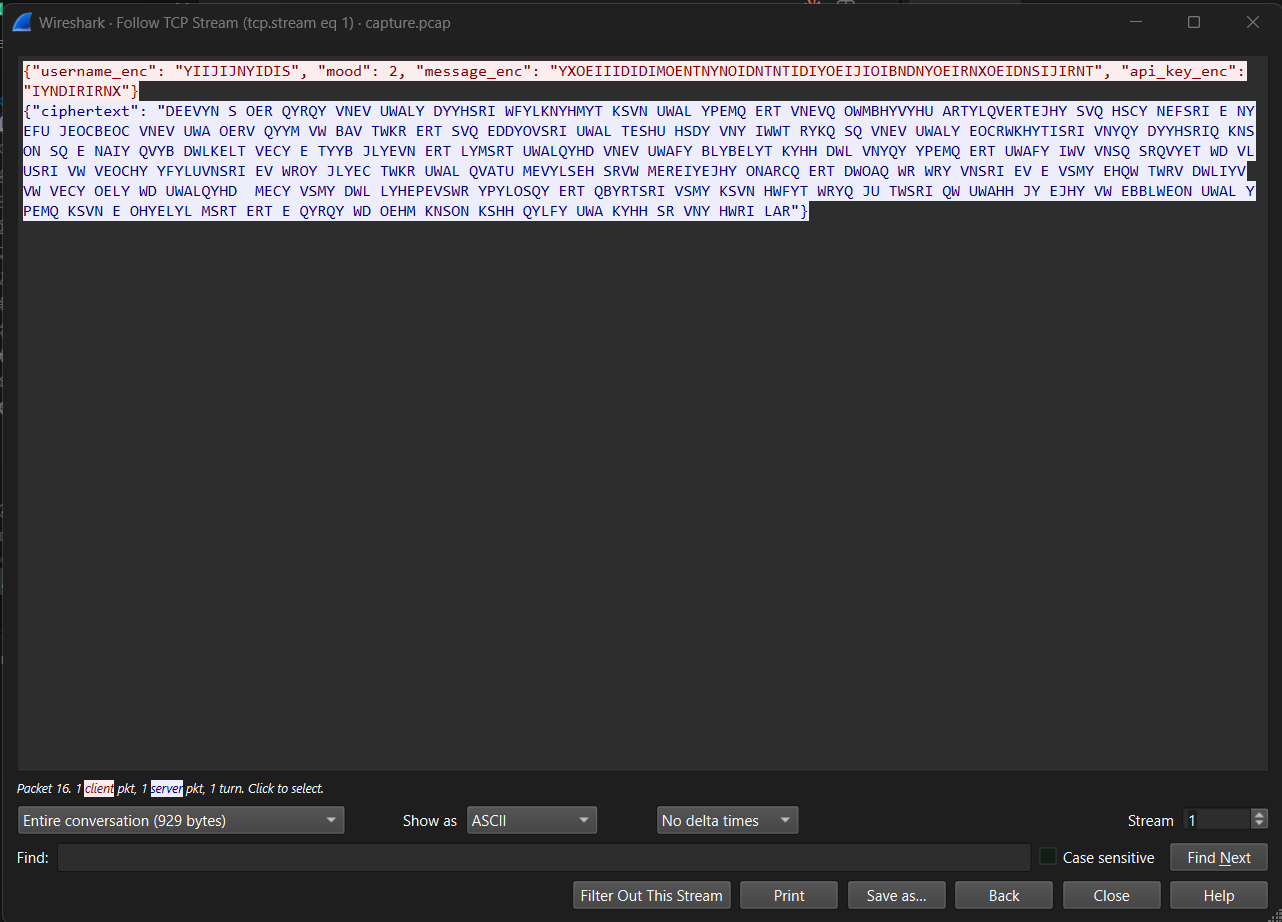
\includegraphics[width=\linewidth]{07_wireshark_stream1.png}
\caption{Stream 1: session 2, mood 2.}\end{subfigure}
\caption{Wireshark \emph{Follow TCP Stream} of the capture: red = \csdir, blue = \scdir.}
\label{fig:wireshark}
\end{figure}

% ================================================================== 2
\section{Frequency Analysis \& Key Recovery}

\subsection{Method}
Letters are numbered $\mathrm{A}=0,\ldots,\mathrm{Z}=25$. The affine cipher and its inverse are
\[
E(x) = (ax + b) \bmod 26, \qquad D(y) = a^{-1}(y - b) \bmod 26,
\]
which needs $\gcd(a,26)=1$, i.e.\ $a \in \{1,3,5,7,9,11,15,17,19,21,23,25\}$: only $12 \times 26 = 312$ keys.

\textbf{Preprocessing.} Only the letters A--Z are counted. JSON syntax, field names, spaces and the occasional stray
space inside \csdir{} ciphertexts are removed. Ciphertexts encrypted under the same mood are pooled (S1 with S3,
C1 with C3), because Section~1 showed that they share a key.

\textbf{Al-Kindi's method.} Every affine key maps each plaintext letter to one fixed cipher letter, so letter
frequencies survive encryption; they are only moved to different letters. The cipher letters are ranked by frequency
and matched against English ranks (E 12.7\%, T 9.1\%, A 8.2\%, O 7.5\%, I 7.0\%, N 6.7\%, \ldots). Each guessed pair of
mappings gives two linear congruences in $a$ and $b$.

\textbf{Testing candidates.} Every solution with $\gcd(a,26)=1$ is used to decrypt the text, and the result is scored
against English with
\[
\chi^2 = \sum_{i=A}^{Z} \frac{(O_i - n p_i)^2}{n p_i},
\]
where $O_i$ is the observed count, $n$ the number of letters and $p_i$ the English frequency. Real English scores in
the tens; wrong keys score in the hundreds or thousands. As an independent check, all 312 keys were also tried
exhaustively.

The tables and charts were generated with \ct{frequency\_analysis.py} (helper \ct{affine.py}); candidate keys were
tested and scored with a companion script built on the same helper.

\subsection{\scdir{} (psychologist replies)}

\begin{figure}[H]\centering
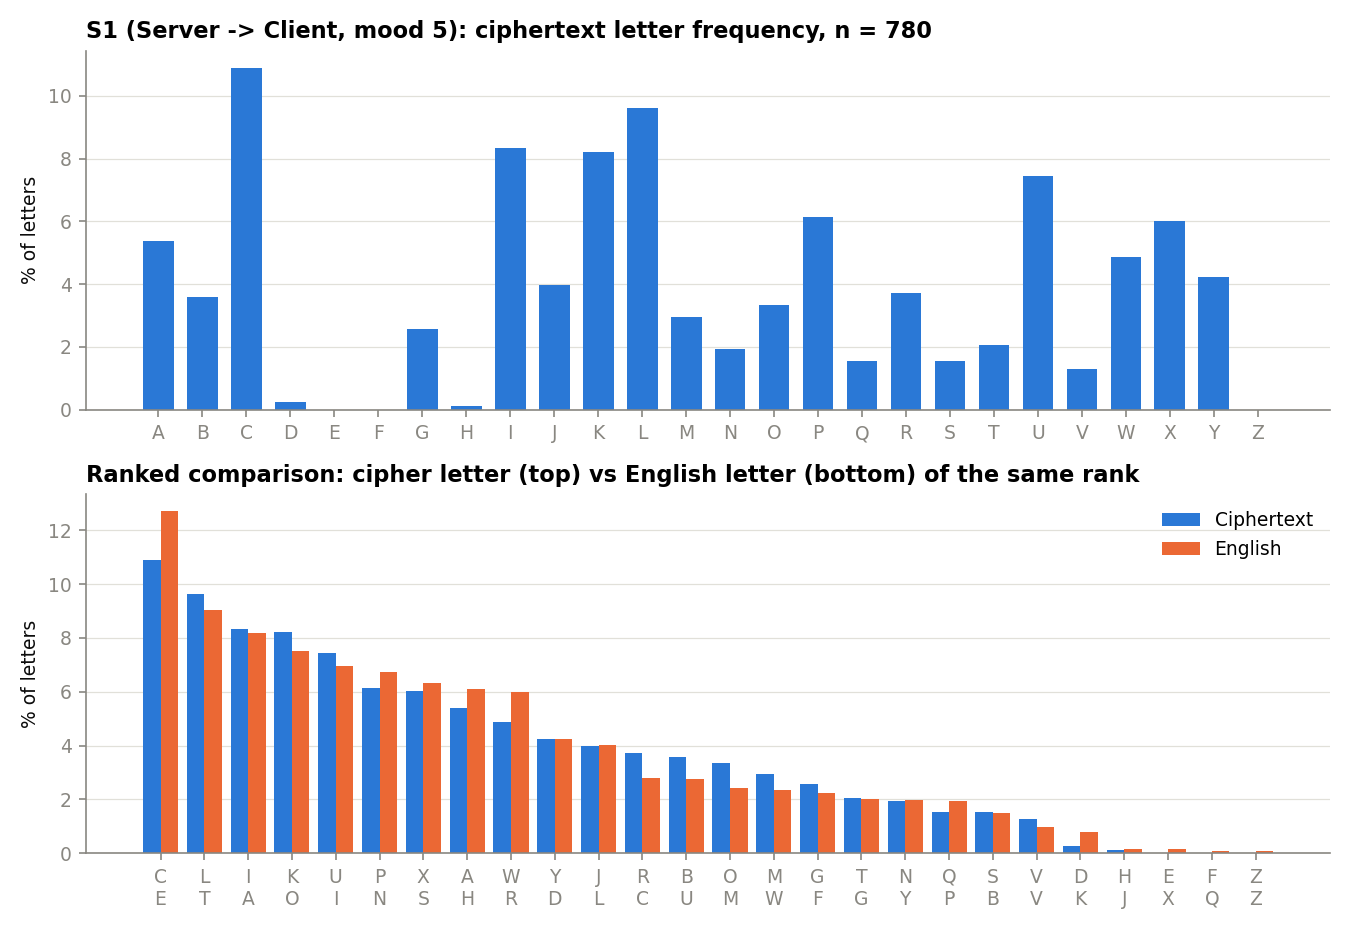
\includegraphics[width=0.92\linewidth]{freq_S1.png}
\caption{S1 (mood 5). Top: cipher letter frequencies. Bottom: cipher letters ranked against English letters of the
same rank (cipher letter above, English letter below). \ct{C} and \ct{L} line up with \ct{E} and \ct{T}.}
\label{fig:freqS1}
\end{figure}

\begin{table}[H]\centering\small
\caption{S1 ranked frequencies ($n = 780$ letters) next to English. Tables for S2--S5 are in Appendix~\ref{app:freq}.}
\begin{tabular}{r c r r c r}
\toprule
Rank & Cipher & Count & \% & English & \% \\
\midrule
\rawinput{data/freq_S1.tex}
\bottomrule
\end{tabular}
\end{table}

The ciphertext distribution has the same shape as English: one letter clearly on top (\ct{C} 10.9\%), a group of
letters at 6--10\%, and a long tail of rare letters (\ct{E}, \ct{F}, \ct{Z} almost absent). This is what a
\emph{monoalphabetic} substitution looks like, and it is exactly what Al-Kindi's method exploits.

\subsubsection*{Mood 5: full working (S1 + S3, 1640 letters)}
Most frequent cipher letters: \ct{C} 11.5\%, \ct{L} 9.9\%, \ct{I} 8.8\%, \ct{K} 7.7\%, \ct{U} 7.1\%.

\textbf{Hypothesis:} $\mathrm{E}\rightarrow\ct{C}$ and $\mathrm{T}\rightarrow\ct{L}$ (the two most common letters in each).
\begin{align*}
4a + b &\equiv 2 \pmod{26} && (\mathrm{E}=4 \rightarrow \ct{C}=2)\\
19a + b &\equiv 11 \pmod{26} && (\mathrm{T}=19 \rightarrow \ct{L}=11)\\
(4-19)\,a &\equiv 2-11 && \text{(subtract)}\\
-15a \equiv -9 \;\Rightarrow\; 11a &\equiv 17 \pmod{26}.
\end{align*}
$\gcd(11,26)=1$, so 11 has an inverse. Extended Euclid:
\begin{align*}
26 &= 2\cdot 11 + 4, \qquad 11 = 2\cdot 4 + 3, \qquad 4 = 1\cdot 3 + 1;\\
1 &= 4 - 3 = 4 - (11 - 2\cdot 4) = 3\cdot 4 - 11\\
  &= 3(26 - 2\cdot 11) - 11 = 3\cdot 26 - 7\cdot 11.
\end{align*}
So $11^{-1} \equiv -7 \equiv 19 \pmod{26}$ (check: $11 \times 19 = 209 = 8\cdot 26 + 1$). Then
\[
a \equiv 19 \times 17 = 323 \equiv \mathbf{11}, \qquad b \equiv 2 - 4\times 11 = -42 \equiv \mathbf{10} \pmod{26}.
\]
$\gcd(11,26)=1$, so the key is valid, and decryption is $D(y) = 19\,(y - 10) \bmod 26$. The result reads
\ct{FAATEH IT SOUNDS LIKE YOURE GOING THROUGH A TOUGH TIME \ldots}, so the key is accepted.

\subsubsection*{Moods 2, 8 and 10}
The same procedure was applied to each mood. When the first guess pairs E with A, the difference $(4-0)=4$ is
\emph{not} invertible mod 26 ($\gcd(4,26)=2$). The congruence is then divided through by 2 and solved mod 13, which
gives two candidates; only the odd one is coprime with 26.

\textbf{Mood 2 (S2, 622 letters).} Top letters \ct{Y} 12.9\%, \ct{E} 9.5\%, \ct{V} 8.2\%. Best mapping:
$\mathrm{E}\rightarrow\ct{Y}$, $\mathrm{A}\rightarrow\ct{E}$.
\begin{align*}
b &\equiv 4 && (\mathrm{A}=0 \rightarrow \ct{E}=4)\\
4a + 4 &\equiv 24 \;\Rightarrow\; 4a \equiv 20 \pmod{26}\\
2a &\equiv 10 \pmod{13} \;\Rightarrow\; a \equiv 5 \pmod{13} \;\Rightarrow\; a \in \{5, 18\}
\end{align*}
Only $a=5$ is coprime with 26, so $\mathbf{(a,b)=(5,4)}$, with $5^{-1} = 21$ ($5\cdot21 = 105 = 4\cdot26+1$).

\textbf{Mood 8 (S4, 666 letters).} Top letters \ct{G} 11.6\%, \ct{B} 10.5\%, \ct{Q} 9.6\%. Mapping
$\mathrm{E}\rightarrow\ct{G}$, $\mathrm{T}\rightarrow\ct{B}$:
\begin{align*}
4a + b &\equiv 6, \qquad 19a + b \equiv 1 \;\Rightarrow\; 11a \equiv 5 \pmod{26}\\
a &\equiv 11^{-1}\times 5 = 19 \times 5 = 95 \equiv 17\\
b &\equiv 6 - 4\times17 = -62 \equiv 16
\end{align*}
So $\mathbf{(a,b)=(17,16)}$, with $17^{-1} = 23$ ($17\cdot 23 = 391 = 15\cdot26+1$).

\textbf{Mood 10 (S5, 672 letters).} Top letters \ct{A} 11.8\%, \ct{U} 9.4\%, \ct{D} 8.9\%. Mapping
$\mathrm{E}\rightarrow\ct{A}$, $\mathrm{A}\rightarrow\ct{U}$:
\begin{align*}
b &\equiv 20 && (\mathrm{A}=0 \rightarrow \ct{U}=20)\\
4a + 20 &\equiv 0 \;\Rightarrow\; 4a \equiv 6 \pmod{26}\\
2a &\equiv 3 \pmod{13} \;\Rightarrow\; a \equiv 3\cdot 7 = 21 \equiv 8 \pmod{13} \;\Rightarrow\; a \in \{8, 21\}
\end{align*}
(using $2^{-1} \equiv 7 \pmod{13}$). Only $a=21$ is coprime with 26, so $\mathbf{(a,b)=(21,20)}$, with $21^{-1} = 5$
($21\cdot 5 = 105 = 4\cdot26+1$).

\subsubsection*{Candidate testing and confirmation}
For each mood, the top cipher letter was mapped to E and the next five cipher letters were each tried as T, A, O, I
and N: 25 hypotheses per mood. Every valid key was scored. The
exhaustive 312-key search agrees in every case, and by a wide margin:

\begin{table}[H]\centering
\caption{Chosen key vs.\ the next-best of all 312 keys (lower $\chi^2$ = closer to English).}
\begin{tabular}{c c c r r}
\toprule
Mood & Winning mappings & Key & $\chi^2$ (key) & $\chi^2$ (runner-up) \\
\midrule
2  & E$\to$\ct{Y}, A$\to$\ct{E} & (5, 4)   & 43.4 & 855.4 \\
5  & E$\to$\ct{C}, T$\to$\ct{L} & (11, 10) & 87.5 & 2183.9 \\
8  & E$\to$\ct{G}, T$\to$\ct{B} & (17, 16) & 39.5 & 940.8 \\
10 & E$\to$\ct{A}, A$\to$\ct{U} & (21, 20) & 31.5 & 953.2 \\
\bottomrule
\end{tabular}
\end{table}

\begin{figure}[H]\centering
\begin{subfigure}{0.49\linewidth}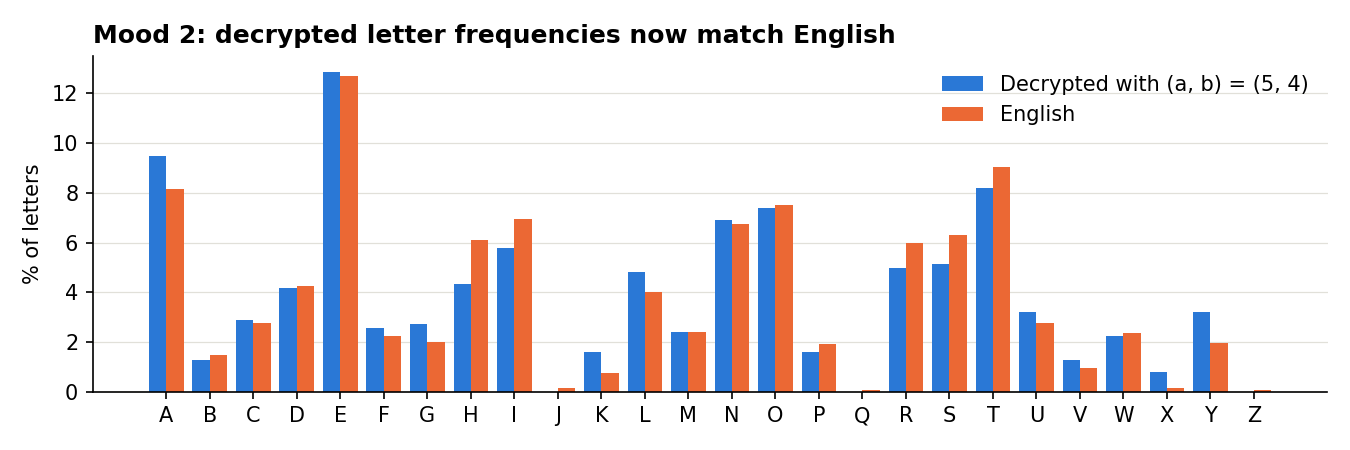
\includegraphics[width=\linewidth]{verify_mood2.png}\end{subfigure}\hfill
\begin{subfigure}{0.49\linewidth}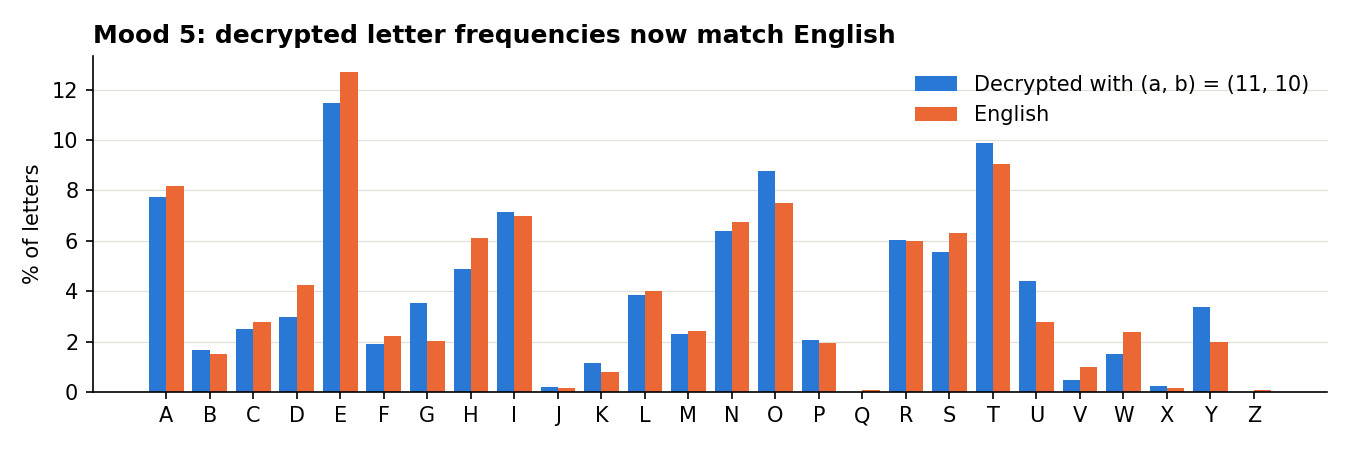
\includegraphics[width=\linewidth]{verify_mood5.png}\end{subfigure}\\[0.4em]
\begin{subfigure}{0.49\linewidth}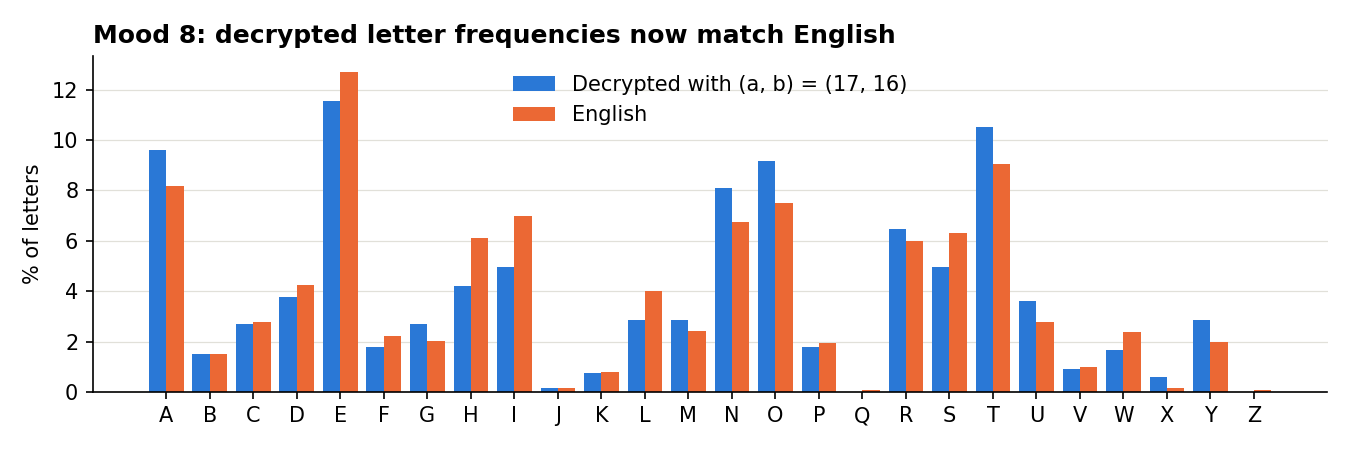
\includegraphics[width=\linewidth]{verify_mood8.png}\end{subfigure}\hfill
\begin{subfigure}{0.49\linewidth}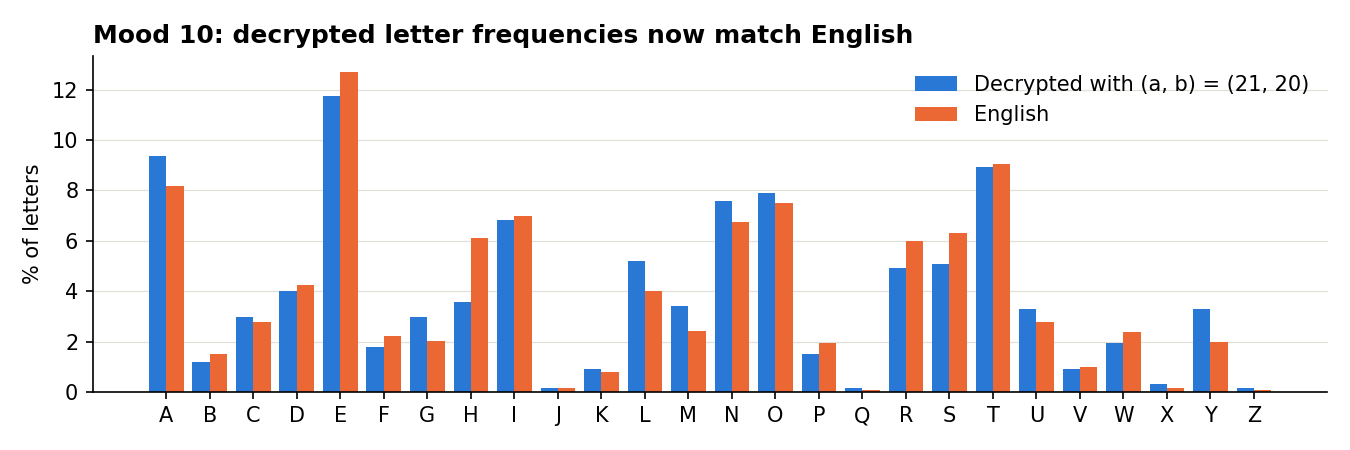
\includegraphics[width=\linewidth]{verify_mood10.png}\end{subfigure}
\caption{After decryption with the recovered keys, letter frequencies (blue) match standard English (orange).}
\end{figure}

\subsection{\csdir{} (patient requests)}

\begin{figure}[H]\centering
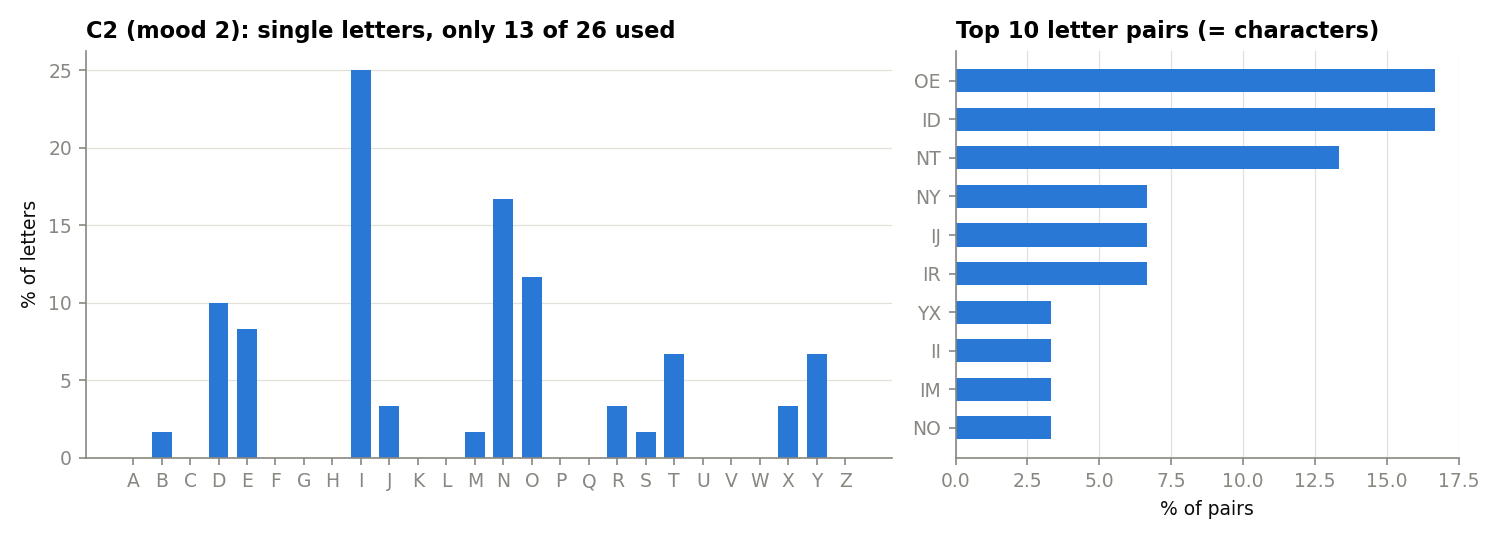
\includegraphics[width=0.95\linewidth]{freq_C2.png}
\caption{C2 (mood 2): only 13 of 26 letters ever appear (left). The letter pairs (right) behave like characters,
with \ct{OE} and \ct{ID} the most common.}
\label{fig:freqC2}
\end{figure}

A normal English ciphertext would use 20--26 different letters. The \csdir{} texts use only \textbf{13--14}, always have
an even length, and \ct{Faateh} (6 characters) becomes 12 letters. Each character is therefore encoded as \textbf{two
symbols from a set of at most 16}, i.e.\ two \textbf{hexadecimal digits} of its ASCII code, and each digit $d \in
\{0,\ldots,15\}$ is then affine-encrypted as a letter. So the unit of frequency analysis is the \emph{pair}.

\textbf{Hypothesis.} The most common character in English text is the \textbf{space}, roughly one character in five.
Its ASCII code is \ct{0x20}, i.e.\ the digits $(2, 0)$. If a pair $\ct{XY}$ is the space then
\[
a \cdot 0 + b \equiv Y \;\Rightarrow\; b = Y, \qquad 2a + b \equiv X \;\Rightarrow\; 2a \equiv X - Y \pmod{26}.
\]
Because $\gcd(2,26)=2$, this has \emph{no} solution when $X-Y$ is odd, and otherwise two solutions $a$ and $a+13$, of
which only the odd one is coprime with 26.

\textbf{Mood 2 (C2).} The top pairs are tied: \ct{ID} and \ct{OE} (16.7\% each).
\begin{itemize}
\item \ct{ID} as space: $b = 3$, $2a \equiv 8-3 = 5$, which is odd, so there is no solution. \textbf{Rejected.}
\item \ct{OE} as space: $b = 4$, $2a \equiv 14-4 = 10 \Rightarrow a \in \{5, 18\}$. $a = 18$ is even, so
      $\mathbf{(a,b)=(5,4)}$. Decrypting gives \ct{I feel stressed about my exams}. \textbf{Accepted.}
\end{itemize}
The rejected pair \ct{ID} is the letter \ct{e} (\ct{0x65}): $5\cdot6+4 = 34 \equiv 8 = \ct{I}$ and
$5\cdot 5+4 = 29 \equiv 3 = \ct{D}$, which fits, since \ct{e} is the most common English letter.

\begin{table}[H]\centering
\caption{\csdir{} key recovery: the most common pair is the space (\ct{0x20}).}
\begin{tabular}{c c c c c c}
\toprule
Mood & Space pair & $b$ & $2a \equiv$ & Candidates & Key \\
\midrule
2  & \ct{OE} (16.7\%) & 4  & 10 & 5, 18  & (5, 4) \\
5  & \ct{GK} (19.0\%) & 10 & 22 & 11, 24 & (11, 10) \\
8  & \ct{YQ} (20.0\%) & 16 & 8  & 4, 17  & (17, 16) \\
10 & \ct{KU} (19.3\%) & 20 & 16 & 8, 21  & (21, 20) \\
\bottomrule
\end{tabular}
\end{table}

For every mood the even candidate is invalid, and the odd one decrypts to readable ASCII.

\subsection{Key schedule}
Putting both directions together:

\begin{table}[H]\centering
\caption{The same key is used in both directions and follows the mood exactly.}
\begin{tabular}{c c c c c}
\toprule
Mood $m$ & \scdir{} key & \csdir{} key & $2m+1$ & $2m$ \\
\midrule
2 & (5, 4) & (5, 4) & 5 & 4 \\
5 & (11, 10) & (11, 10) & 11 & 10 \\
8 & (17, 16) & (17, 16) & 17 & 16 \\
10 & (21, 20) & (21, 20) & 21 & 20 \\
\bottomrule
\end{tabular}
\end{table}

\[
\boxed{\,a = 2m + 1, \qquad b = 2m \pmod{26}\,}
\]

This held for all four moods tested. One consequence is that mood $m = 6$ would give $a = 13$, which is not coprime with
26 and so cannot be decrypted uniquely. That mood was not tested. All sessions used the username \ct{Faateh}, so this
data shows no influence of the username on the key.

% ================================================================== 3
\section{Decryption Results}

\subsection{Worked example: \scdir{} (S1, mood 5)}
Key $(11,10)$, $a^{-1}=19$, $D(y) = 19(y-10) \bmod 26$. First word \ct{NKKLCJ}:

\begin{table}[H]\centering
\begin{tabular}{c c c c c}
\toprule
Cipher & $y$ & $19(y-10)$ & mod 26 & Plain \\
\midrule
\ct{N} & 13 & 57   & 5  & \ct{F} \\
\ct{K} & 10 & 0    & 0  & \ct{A} \\
\ct{K} & 10 & 0    & 0  & \ct{A} \\
\ct{L} & 11 & 19   & 19 & \ct{T} \\
\ct{C} & 2  & $-152$ & 4  & \ct{E} \\
\ct{J} & 9  & $-19$  & 7  & \ct{H} \\
\bottomrule
\end{tabular}
\end{table}

\subsection{Worked example: \csdir{} (C2, mood 2)}
Key $(5,4)$, $a^{-1}=21$. Each letter gives a hex digit $d = 21(y-4) \bmod 26$, and each pair of digits gives one
character:

\begin{table}[H]\centering
\begin{tabular}{c c c c c}
\toprule
Letters & $y$ & Digits $21(y-4) \bmod 26$ & Hex & Character \\
\midrule
\ct{Y X} & 24, 23 & 4, 9 & \ct{0x49} & \ct{I} \\
\ct{O E} & 14, 4  & 2, 0 & \ct{0x20} & (space) \\
\ct{I I} & 8, 8   & 6, 6 & \ct{0x66} & \ct{f} \\
\bottomrule
\end{tabular}
\end{table}

\subsection{All ciphertexts}

\begin{table}[H]\centering\small
\caption{All 10 ciphertexts decrypted. Full replies are in Appendix~\ref{app:plain}.}
\begin{tabularx}{\textwidth}{c c c X}
\toprule
ID & Mood & Key & Plaintext \\
\midrule
C1 & 5  & (11, 10) & I have not been sleeping well and I feel tired all the time \\
C2 & 2  & (5, 4)   & I feel stressed about my exams \\
C3 & 5  & (11, 10) & My friends have been ignoring me lately and I feel lonely \\
C4 & 8  & (17, 16) & I got a good grade but I still worry about the next semester \\
C5 & 10 & (21, 20) & I feel great today and want tips to keep my motivation up \\
\midrule
S1 & 5  & (11, 10) & \ct{FAATEH IT SOUNDS LIKE YOURE GOING THROUGH A TOUGH TIME RIGHT NOW} \ldots \\
S2 & 2  & (5, 4)   & \ct{FAATEH I CAN SENSE THAT YOURE FEELING OVERWHELMED WITH YOUR EXAMS} \ldots \\
S3 & 5  & (11, 10) & \ct{FAATEH IT SOUNDS LIKE YOURE FEELING A BIT ISOLATED RIGHT NOW} \ldots \\
S4 & 8  & (17, 16) & \ct{FAATEH IT SOUNDS LIKE YOURE FEELING A BIT ANXIOUS ABOUT NOT} \ldots \\
S5 & 10 & (21, 20) & \ct{FAATEH IT SOUNDS LIKE YOURE FEELING INCREDIBLY MOTIVATED} \ldots \\
\bottomrule
\end{tabularx}
\end{table}

Every decrypted request matches exactly what was typed into the client. The other encrypted request fields decrypt
too:

\begin{table}[H]\centering\small
\begin{tabular}{c l l l l}
\toprule
Mood & \ct{username\_enc} & Plain & \ct{api\_key\_enc} & Plain \\
\midrule
2  & \ct{YIIJIJNYIDIS} & Faateh & \ct{IYNDIRIRNX} & dummy \\
5  & \ct{CYYVYVJCYNYU} & Faateh & \ct{YCJNYXYXJF} & dummy \\
8  & \ct{GOOHOHFGOXOW} & Faateh & \ct{OGFXODODFN} & dummy \\
10 & \ct{AQQPQPLAQVQG} & Faateh & \ct{QALVQHQHLB} & dummy \\
\bottomrule
\end{tabular}
\end{table}

A real API key typed into this client would be exposed in exactly the same way.

A general decryption script was also written for any PsycoSupport ciphertext. Given the mood it applies $a=2m+1$, $b=2m$;
without a mood it searches all 312 keys. Run blind over \ct{ciphertexts.csv}, it recovered all 10 keys, and every
one matched the key schedule.

\subsection{Validation: an Ollama-backed \texttt{server.py}}
\label{sec:ownserver}
As a final check that the recovered protocol is complete, the server was rebuilt from it alone as
\ct{server.py} (submitted). It listens on port 9999 and decrypts the request fields (hex layer, then
$a = 2m+1$, $b = 2m$). It asks the local \ct{llama3.2} model for advice directly, without Groq or the relay. It then
upper-cases the reply, keeps only letters and spaces, and affine-encrypts it with the same key.

Two tests were run:
\begin{enumerate}
\item \textbf{Replay of real traffic.} The exact request bytes of session~1, taken from the capture, were sent to
      \ct{server.py}. It logged \ct{user=Faateh mood=5 msg\_len=59}, identical to the original server's log for that
      request, and its reply began \ct{NKKLCJ \ldots}, the same opening as S1.
\item \textbf{The original client against the new server, at an unseen mood.} The unmodified \ct{client} was used
      with mood \textbf{3}, a mood never captured, whose predicted key is $(a,b) = (7,6)$. The client decrypted the
      reply correctly (Figure~\ref{fig:ownserver}), which confirms the key schedule on a new mood.
\end{enumerate}

\begin{figure}[H]\centering
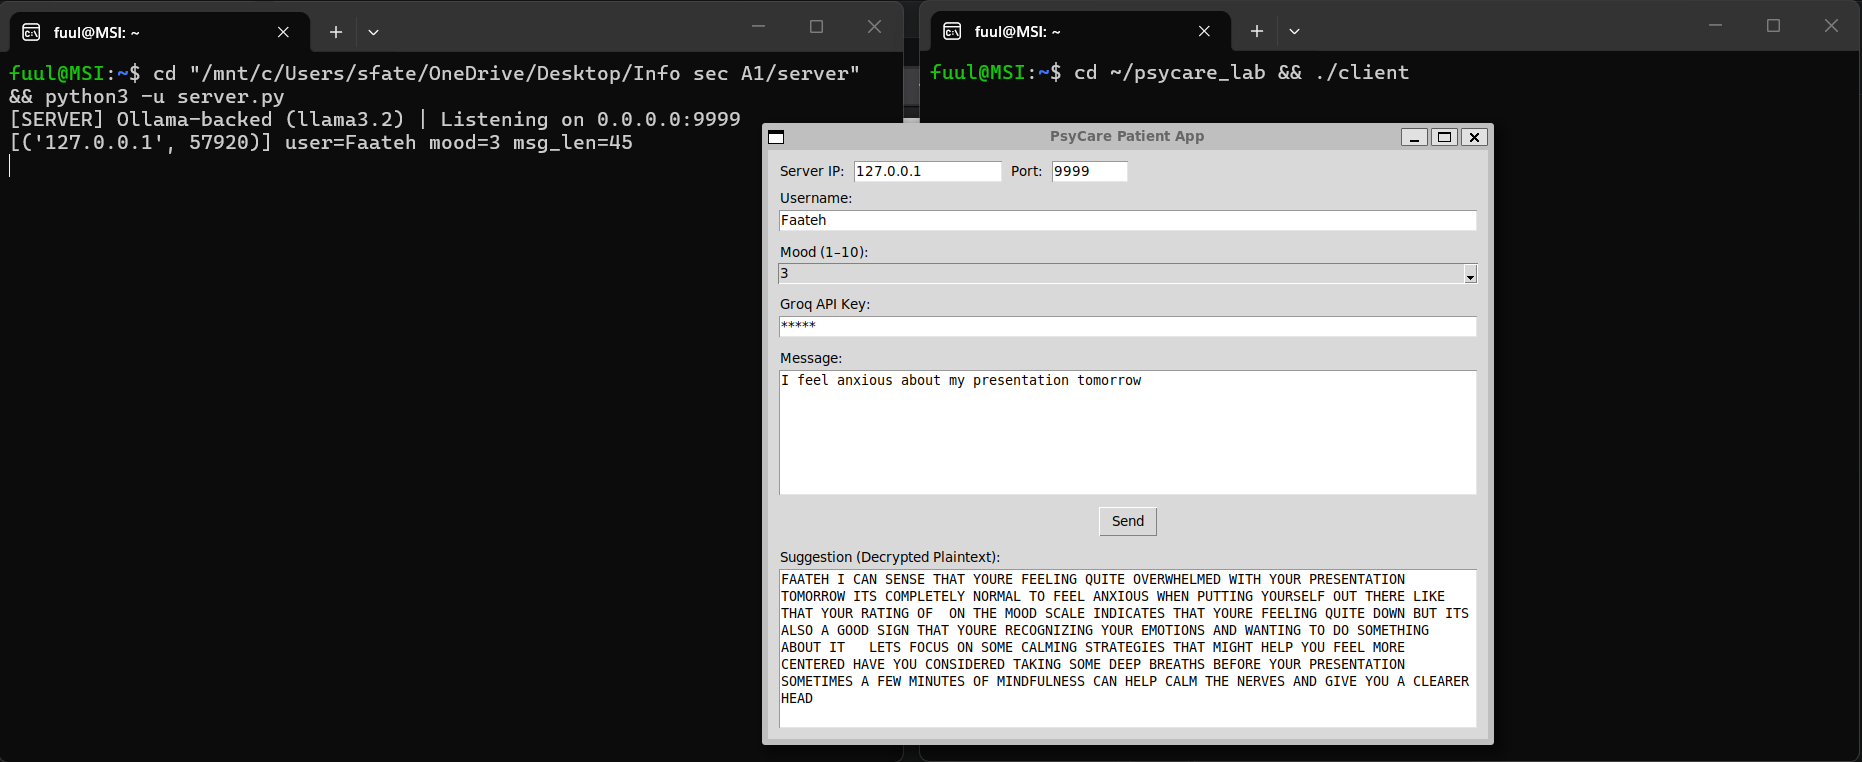
\includegraphics[width=\linewidth]{own_server_test.png}
\caption{The original PsycoSupport client talking to the re-implemented, Ollama-backed \ct{server.py} at mood 3.
The digit ``3'' in the model's reply (``your rating of 3'') is dropped because the protocol carries only letters and
spaces, the same behaviour as the original server.}
\label{fig:ownserver}
\end{figure}

% ================================================================== 4
\section{Security Analysis \& Reflection}

\subsection{Why LLM output makes a classical cipher easy to break}
\begin{itemize}
\item \textbf{Long, natural English.} Each reply is 600--1000 letters of ordinary prose, far more than the roughly
      100 letters frequency analysis needs. The statistics converge on English (Figure~\ref{fig:freqS1}).
\item \textbf{Boilerplate and a fixed opening.} Four of the five replies begin \ct{FAATEH IT SOUNDS LIKE YOURE
      FEELING}. The username is always the first word: a guaranteed \emph{known plaintext}. Two letters are enough:
      from \ct{NKKLCJ} $=$ \ct{FAATEH}, A$\to$\ct{K} gives $b=10$, and F$\to$\ct{N} gives $5a+10\equiv13
      \Rightarrow a \equiv 3\cdot 21 = 63 \equiv 11$. That is the full key without any statistics.
\item \textbf{Formatting leaks structure.} The reply is upper-cased with punctuation removed, but spaces are kept, so
      word lengths, one-letter words (\ct{A}, \ct{I}) and repeated words (\ct{YOU}, \ct{THE}, \ct{AND}) are visible.
\item \textbf{Predictable requests.} Client messages are short, but the space character (about 20\% of characters)
      and the fixed hex layout give two equations immediately.
\end{itemize}

\subsection{Design flaws beyond the cipher}
\begin{enumerate}
\item \textbf{Tiny keyspace:} 312 keys can be tried in milliseconds.
\item \textbf{The key is public:} it is derived from the mood ($a=2m+1$, $b=2m$), and the mood is sent in plaintext
      in every request. Once the schedule is known, no cryptanalysis is needed at all.
\item \textbf{Same key in both directions} doubles the material available to an attacker for each key.
\item \textbf{The hex layer is encoding, not encryption.} It adds no secret, and its 16-symbol alphabet makes the
      ciphertext \emph{more} recognisable.
\item \textbf{No integrity or authentication:} an attacker can change the mood or the ciphertext in transit and
      nothing detects it.
\item \textbf{Secrets under the weak cipher:} the API key is protected only by the same affine cipher.
\item \textbf{Wide binding:} the server listens on \ct{0.0.0.0:9999}, i.e.\ on every network interface, not only on
      loopback.
\item \textbf{Plaintext internal hops:} the server sends the decrypted concern to the model unencrypted (via the relay
      here, or Groq originally).
\end{enumerate}

\subsection{Recommended alternatives (implemented and tested)}
\label{sec:fixes}
Both fixes recommended in the handout were built as a small, separate proof of concept. It does
the same job (username, mood and concern in; advice from the local \ct{llama3.2} out) without touching the lab
programs.

\begin{enumerate}
\item \textbf{TLS 1.3 with a self-signed certificate} (\ct{--mode tls}, port 9443). Python's \ct{ssl} module with
      \ct{minimum\_version = TLSv1\_3}. The client trusts only the server's certificate (pinned with \ct{cafile}) and
      checks the hostname, so a man-in-the-middle with a different certificate is rejected. The negotiated cipher was
      \ct{TLS\_AES\_256\_GCM\_SHA384} (authenticated encryption). A client limited to TLS~1.2 was refused with
      \ct{PROTOCOL\_VERSION}.
\item \textbf{UNIX domain socket} (\ct{--mode unix}). The server listens on a socket \emph{file},
      \ct{\textasciitilde/psycare\_secure/psycare.sock}, with permissions \ct{0600} (\ct{srw-------}). The traffic
      never enters the network stack, so packet sniffers cannot see it, and the operating system blocks other users
      from connecting. The certificate's private key is also \ct{0600} and lives outside the project.
\end{enumerate}

\textbf{Same attack, repeated.} \ct{tcpdump} captured loopback (excluding Ollama's main port) while
a demo script sent three messages over each channel. An analysis script then ran the
eavesdropper's analysis on both captures:

\begin{table}[H]\centering\small
\caption{What an eavesdropper gets: original channel vs.\ TLS 1.3.}
\begin{tabular}{l c c}
\toprule
 & Original (port 9999) & TLS 1.3 demo (port 9443) \\
\midrule
Structure visible & JSON keys, \ct{"mood": N} & none \\
Username / concern words in packets & no (but broken by analysis) & no \\
Symbols seen & 23 letters A--Z (S1) & 256 of 256 byte values \\
Shannon entropy & 4.18 bits/letter (English $\approx$ 4.1) & 7.96 bits/byte (max 8) \\
Frequency analysis & key recovered, all text read & nothing to map \\
\bottomrule
\end{tabular}
\end{table}

\begin{figure}[H]\centering
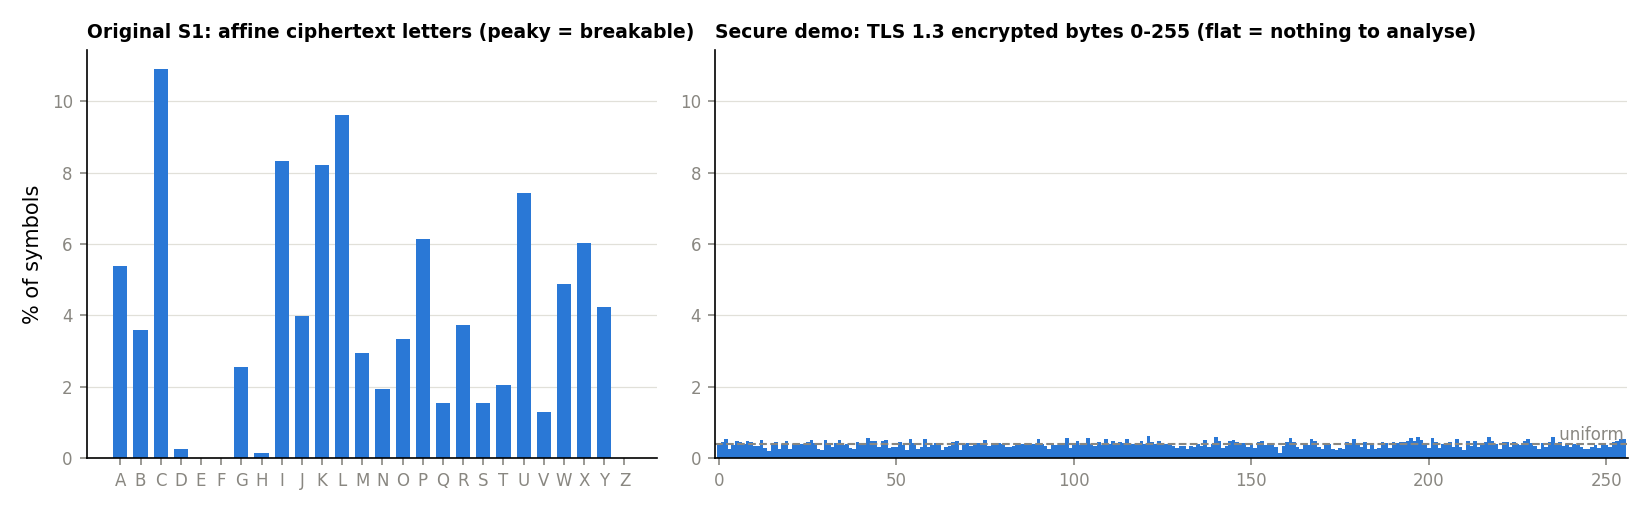
\includegraphics[width=\linewidth]{secure_vs_original.png}
\caption{Left: affine ciphertext keeps the uneven, English-like shape that frequency analysis exploits. Right: TLS~1.3
encrypted bytes are essentially uniform (same vertical scale).}
\end{figure}

\begin{figure}[H]\centering
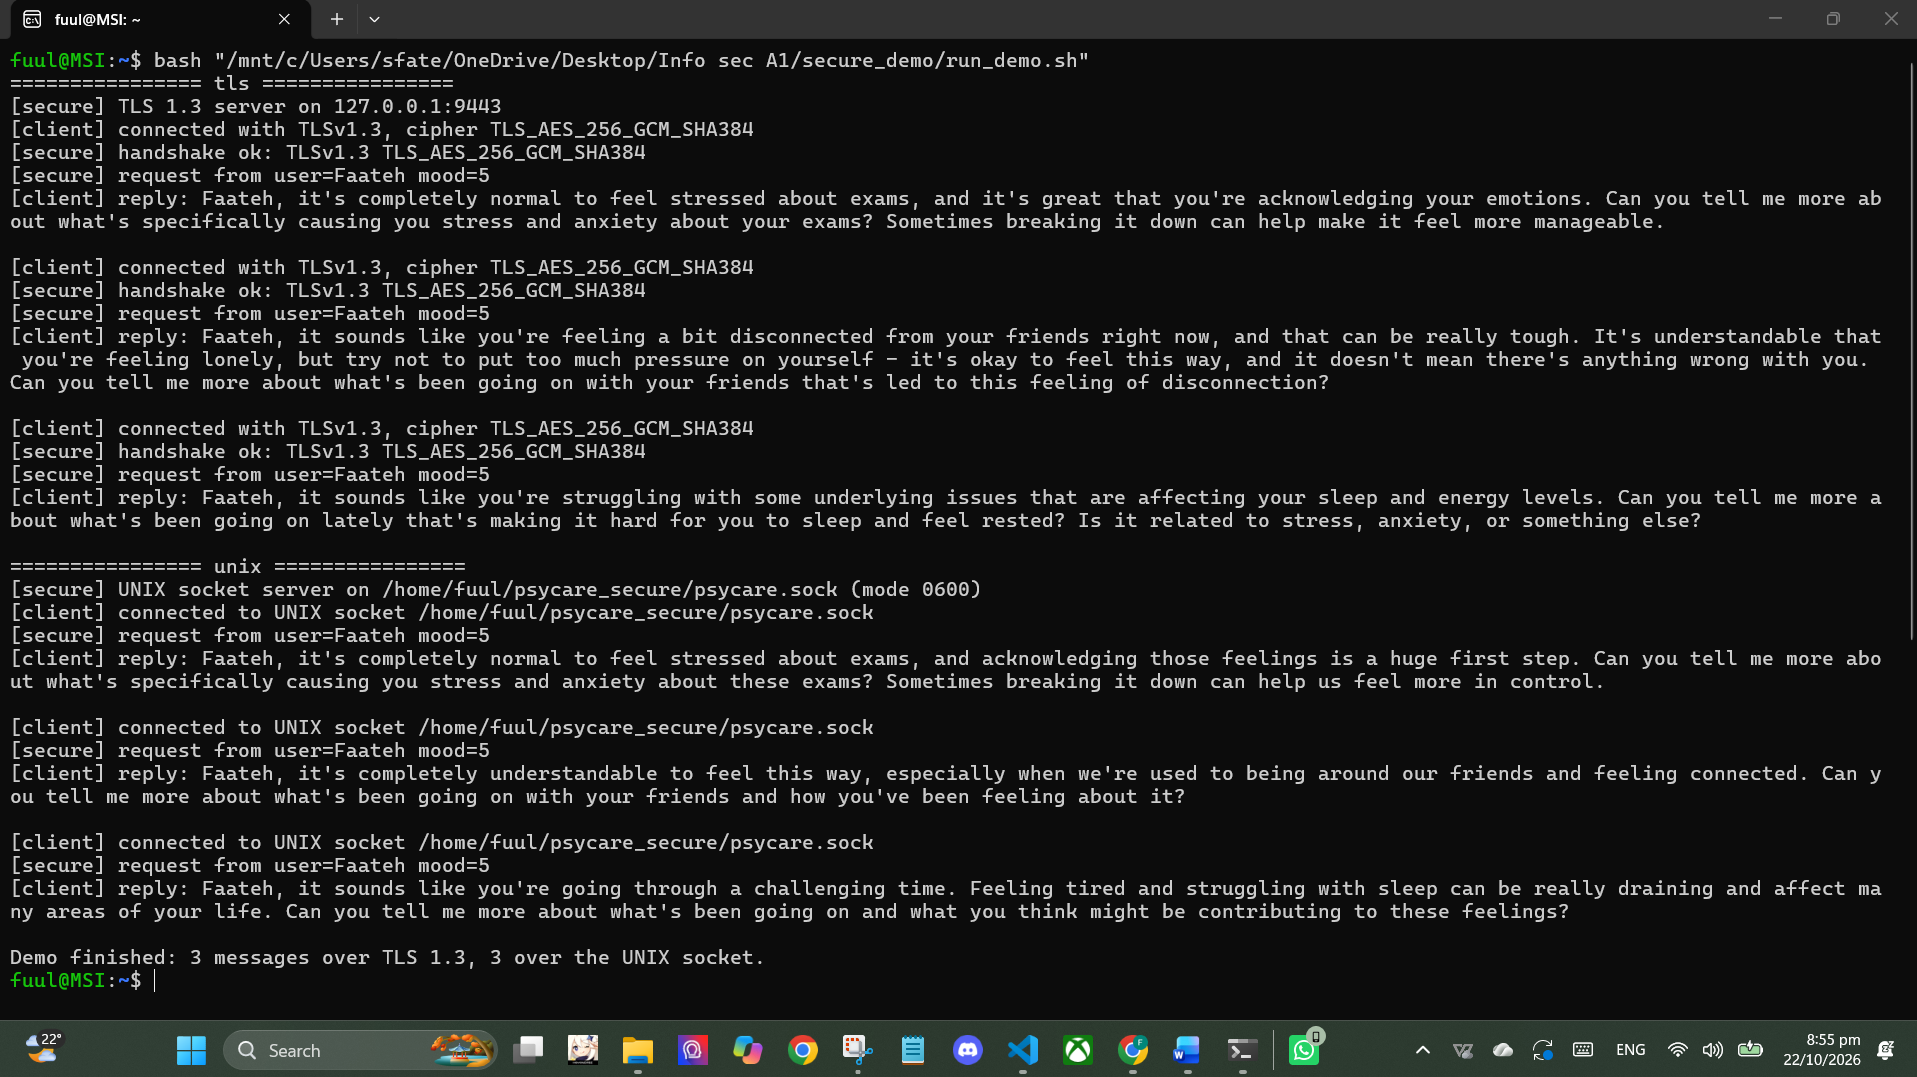
\includegraphics[width=0.85\linewidth]{09_secure_demo_run.png}
\caption{Secure demo: three exchanges over TLS 1.3 and three over the UNIX socket, captured with \ct{tcpdump}
running alongside.}
\end{figure}

\textbf{The UNIX socket exchange never appeared in the capture:} no packet contained the client's
\ct{"username"} request.

\textbf{An important limitation found.} The capture also contained 81{,}893 bytes on a random loopback port
(39237): Ollama's \emph{internal model runner}. Ollama forwards each prompt to it over plain HTTP, and the packets
contained \ct{Patient Faateh, mood 5/10: I feel stressed about my exams} in clear text. Protecting the client--server
channel alone is therefore not enough. \textbf{Every hop that carries patient data needs protection}, including
server$\rightarrow$LLM. Options include running the model in-process, using only owner-restricted local IPC, or
isolating the inference service in its own namespace or container. The same applies to the original lab, whose
server$\rightarrow$relay$\rightarrow$Ollama hop is unencrypted.

Further recommendations: never derive keys from user-visible input, use authenticated encryption, do not send API
keys from the client at all (keep them server-side), and bind services to \ct{127.0.0.1} or a socket file rather
than \ct{0.0.0.0}.

\subsection{Reflection}

\textbf{(a) Input influence.}
The \emph{mood} completely determines the key. The same mood produced identical ciphertext openings (S1 and S3), and
every other mood gave a different key ($a=2m+1$, $b=2m$). The \emph{concern} changes the plaintext and therefore the
ciphertext, and it also shapes the reply: worried concerns gave replies that open with ``it sounds like you're going
through a tough time'' or ``feeling a bit anxious'', while the positive one opened with ``incredibly motivated''. The
\emph{username} appears as the first word of every reply, so it leaks a known plaintext rather than changing the key.
Only one username was used, as the handout requires.

\textbf{(b) Communication direction.}
The two directions use the same key but different encodings. \scdir{} encrypts upper-case letters and keeps spaces, so
the text looks like scrambled English and gives way to single-letter analysis. \csdir{} hex-encodes each character first,
so it is twice as long, has no word breaks, uses at most 16 letters, and needs analysis of letter \emph{pairs}
instead. Requests are short (30--60 characters), while replies are long (600--1000 letters), so the replies carry far
more statistical evidence. In practice the replies leak the key, and that key then unlocks the requests.

\textbf{(c) Cryptographic behaviour.}
Frequency analysis showed that the cipher is monoalphabetic: every key just relabels the English distribution, which
survives intact (Figure~\ref{fig:freqS1}). With only 312 keys, a key that is derived from public data and the same in
both directions, and highly regular LLM text, the scheme falls to both ciphertext-only and known-plaintext attacks
within seconds. It gives a false sense of security: the traffic looks scrambled but protects nothing. A 9th-century
technique was enough to break a 2026 application, which is why systems must use vetted modern protocols such as
TLS~1.3 rather than home-made ciphers.

\textbf{(d) Ethical considerations.}
This work was authorised and contained. It used only the instructor's PsycoSupport build, on a machine I control,
over the loopback interface, with synthetic concerns and a dummy API key. No real patient or third party was
involved. The same interception against a real application or real users without permission would be illegal (for
example under Pakistan's Prevention of Electronic Crimes Act 2016 on unauthorised access and interception) and a
serious breach of privacy. Mental-health conversations are among the most sensitive data a person can share, and
exposing them could cause real harm. The skills are the same, so the deciding factors are \emph{authorisation, scope
and intent}. Penetration testers work under written permission, stay within agreed limits, and report weaknesses
responsibly so they can be fixed, which is what Section~\ref{sec:fixes} does for this application.

% ================================================================== 5
\section{Submitted Files \& Environment}

The submission contains everything needed to rerun the work on a machine with Ollama and \ct{llama3.2}. Step-by-step
commands are in the included \ct{README.md}.

\begin{table}[H]\centering
\begin{tabularx}{\textwidth}{l X}
\toprule
File & Contents \\
\midrule
\ct{23I-0688-FaatehHaneef-A1.pdf} & This report. \\
\ct{README.md}, \ct{requirements.txt} & How to rerun every step; Python dependency (matplotlib). \\
\ct{ciphertexts.csv} & All 10 captured ciphertexts: ID, session, direction, mood, length, ciphertext, and the
                       encrypted username and API-key fields. \\
\ct{evidence/capture.pcap} & The original loopback capture (Section~1). \\
\ct{server/server.py} & PsycoSupport server re-implemented with a local Ollama backend; same protocol, works with the
                 original client (Section~\ref{sec:ownserver}). \\
\ct{scripts/relay.py} & Groq$\rightarrow$Ollama bridge that let the unmodified original \ct{server} run offline during
                capture (Section~1.1). \\
\ct{scripts/extract\_ciphertexts.py} & Reassembles the TCP streams in a \ct{.pcap} and writes \ct{ciphertexts.csv}. \\
\ct{scripts/frequency\_analysis.py} & Frequency tables and charts (Section~2). \\
\ct{scripts/crack\_keys.py} & Key recovery: hypotheses, congruences, inverses, $\chi^2$ testing, decryptions. \\
\ct{scripts/decrypt.py} & General decryptor for any mood and direction (Section~3). \\
\ct{scripts/affine.py} & Shared affine-cipher maths and English frequencies. \\
\ct{secure\_demo/}, \ct{evidence/secure\_capture.pcap} & TLS~1.3 and UNIX-socket fixes, demo script, and the
                attack rerun against them (Section~\ref{sec:fixes}). \\
\bottomrule
\end{tabularx}
\end{table}

Rerunning the analysis from the provided capture:
\begin{lstlisting}
python3 scripts/extract_ciphertexts.py evidence/capture.pcap ciphertexts.csv
python3 scripts/frequency_analysis.py ciphertexts.csv output
python3 scripts/crack_keys.py ciphertexts.csv output
python3 scripts/decrypt.py --csv ciphertexts.csv
\end{lstlisting}

\textbf{Environment.}
\begin{itemize}
\item \textbf{Platform:} Ubuntu 24.04 under WSL2 (Windows 11), NVIDIA RTX 3050 Ti; Ollama 0.40.4 serving
      \ct{llama3.2}; the supplied \ct{client} and \ct{server} executables, unmodified.
\item \textbf{Capture:} \ct{tcpdump} 4.99 on the loopback interface; Wireshark 4.6 for \emph{Follow TCP Stream}.
\item \textbf{Analysis:} Python 3 (standard library) with matplotlib for the charts.
\end{itemize}

% ------------------------------------------------------------------ references
\section*{References}
\addcontentsline{toc}{section}{References}
\begin{enumerate}[label={[\arabic*]}]
\item Al-Kindi, \emph{A Manuscript on Deciphering Cryptographic Messages}, 9th century. Summarised in S.~Singh,
      \emph{The Code Book}, Fourth Estate, 1999.
\item R.~E.~Lewand, \emph{Cryptological Mathematics}, Mathematical Association of America, 2000 (English letter
      frequencies).
\item D.~R.~Stinson, M.~B.~Paterson, \emph{Cryptography: Theory and Practice}, 4th ed., CRC Press, 2018 (affine cipher,
      extended Euclidean algorithm).
\item E.~Rescorla, \emph{The Transport Layer Security (TLS) Protocol Version 1.3}, RFC 8446, IETF, 2018.
\item Python Software Foundation, \emph{ssl --- TLS/SSL wrapper for socket objects}, Python 3 documentation.
\item Linux man-pages, \emph{unix(7) --- sockets for local interprocess communication}.
\item Ollama, documentation and OpenAI-compatible API, \url{https://github.com/ollama/ollama}.
\item Government of Pakistan, \emph{Prevention of Electronic Crimes Act}, 2016.
\item M.~A.~Rehman, PsycoSupport lab repository, \url{https://github.com/maadilrehman/PsycoSupport}.
\end{enumerate}

% ------------------------------------------------------------------ appendices
\appendix
\newpage
\section{Full decrypted replies}
\label{app:plain}

\subsection*{S1 (mood 5, key (11, 10))}
{\small\ttfamily\raggedright \input{data/plain_S1.txt}}

\subsection*{S2 (mood 2, key (5, 4))}
{\small\ttfamily\raggedright \input{data/plain_S2.txt}}

\subsection*{S3 (mood 5, key (11, 10))}
{\small\ttfamily\raggedright \input{data/plain_S3.txt}}

\subsection*{S4 (mood 8, key (17, 16))}
{\small\ttfamily\raggedright \input{data/plain_S4.txt}}

\subsection*{S5 (mood 10, key (21, 20))}
{\small\ttfamily\raggedright \input{data/plain_S5.txt}}

\newpage
\section{Frequency tables and charts}
\label{app:freq}

\newcommand{\freqtable}[3]{%
\begin{table}[H]\centering\small
\caption{#1 (mood #2) ranked frequencies, $n = #3$ letters.}
\begin{tabular}{r c r r c r}
\toprule
Rank & Cipher & Count & \% & English & \% \\
\midrule
\rawinput{data/freq_#1.tex}
\bottomrule
\end{tabular}
\end{table}}

% one page per ciphertext: chart first, then its own table
\begin{figure}[H]\centering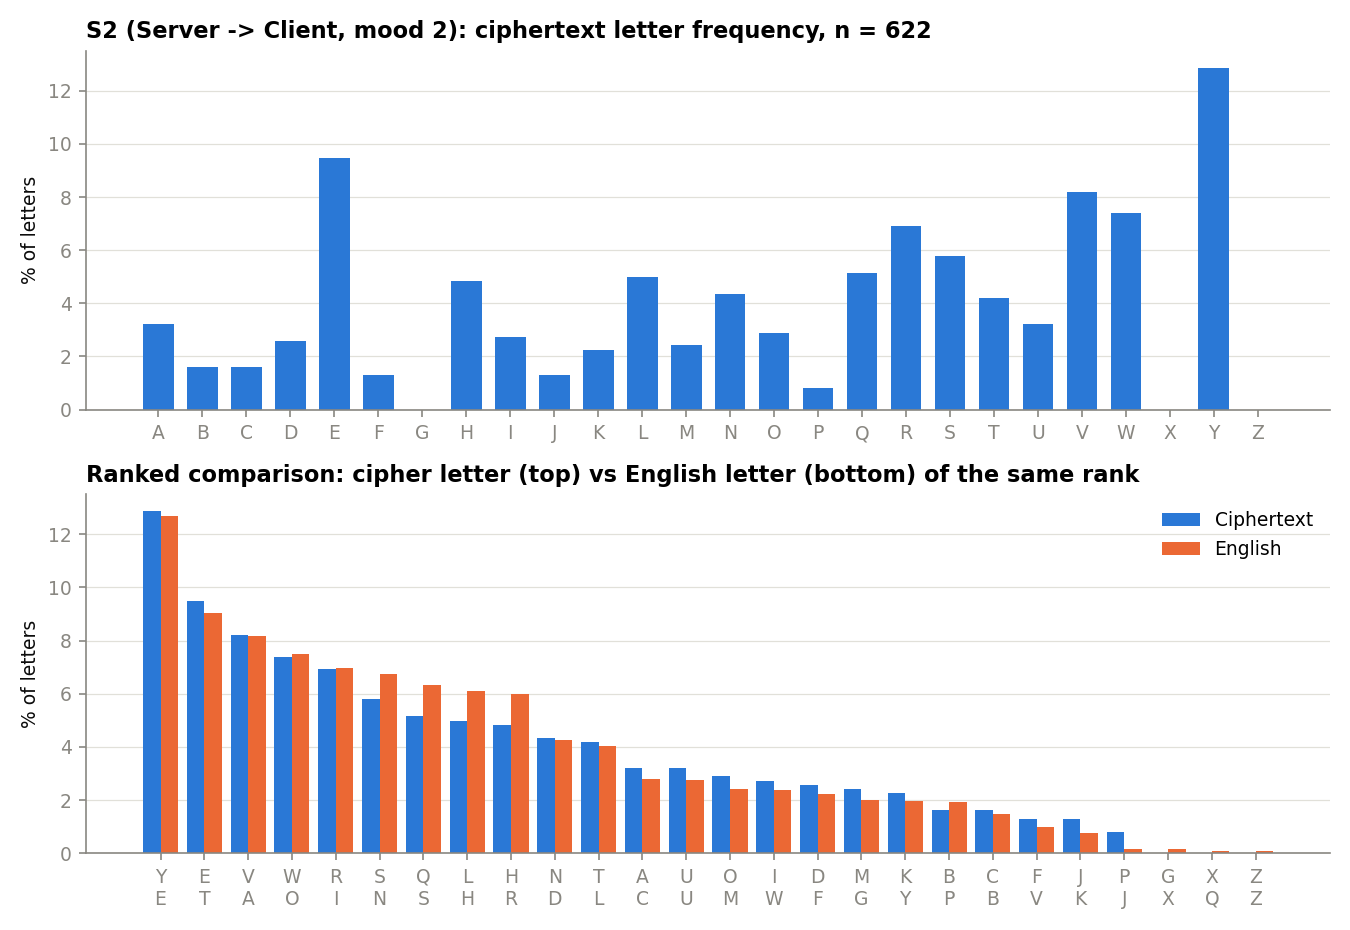
\includegraphics[width=0.8\linewidth]{freq_S2.png}\caption{S2 (mood 2).}\end{figure}
\freqtable{S2}{2}{622}
\clearpage
\begin{figure}[H]\centering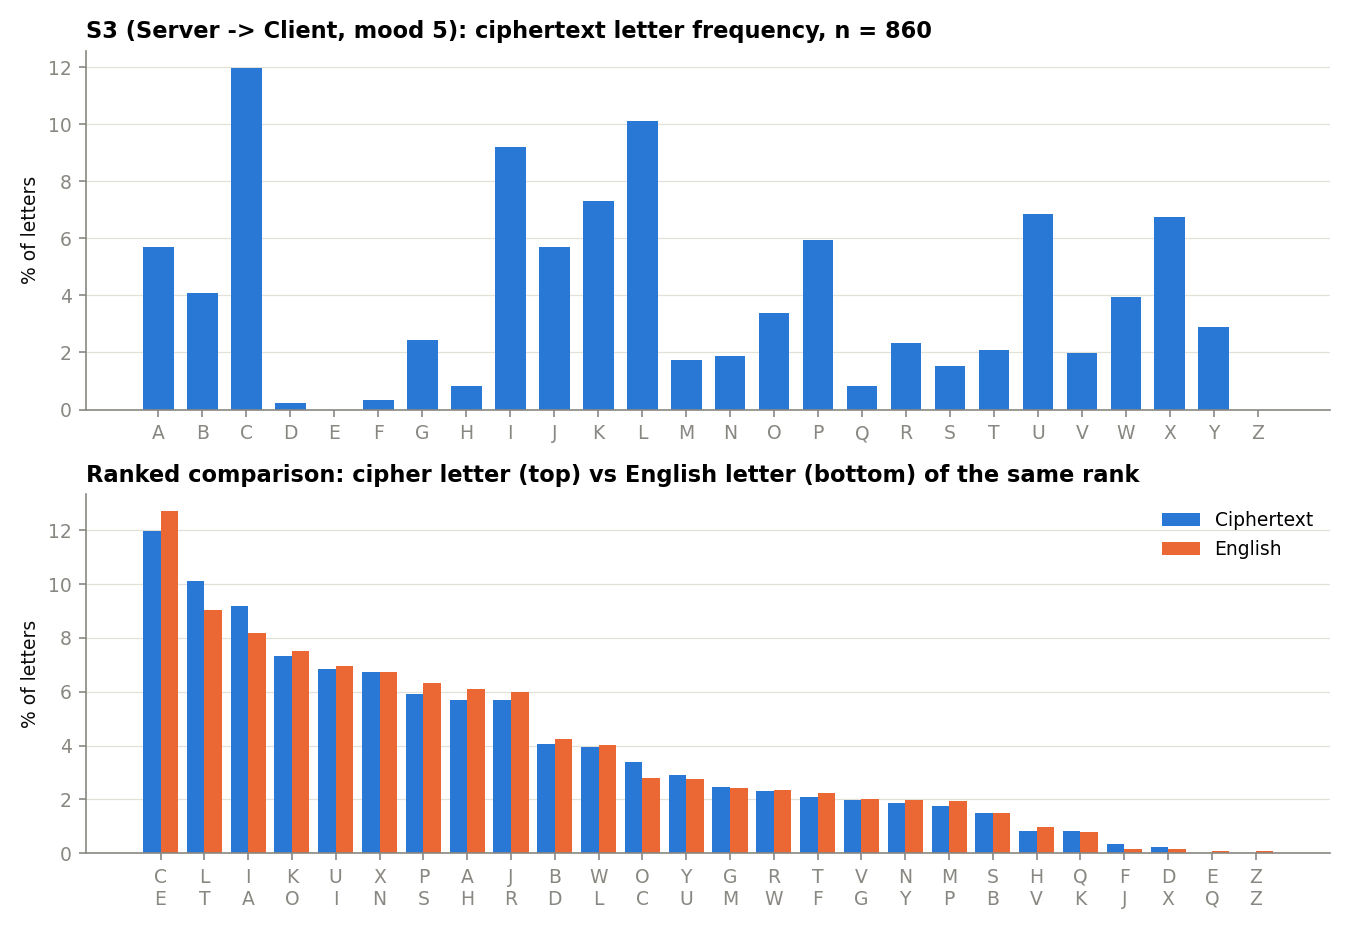
\includegraphics[width=0.8\linewidth]{freq_S3.png}\caption{S3 (mood 5).}\end{figure}
\freqtable{S3}{5}{860}
\clearpage
\begin{figure}[H]\centering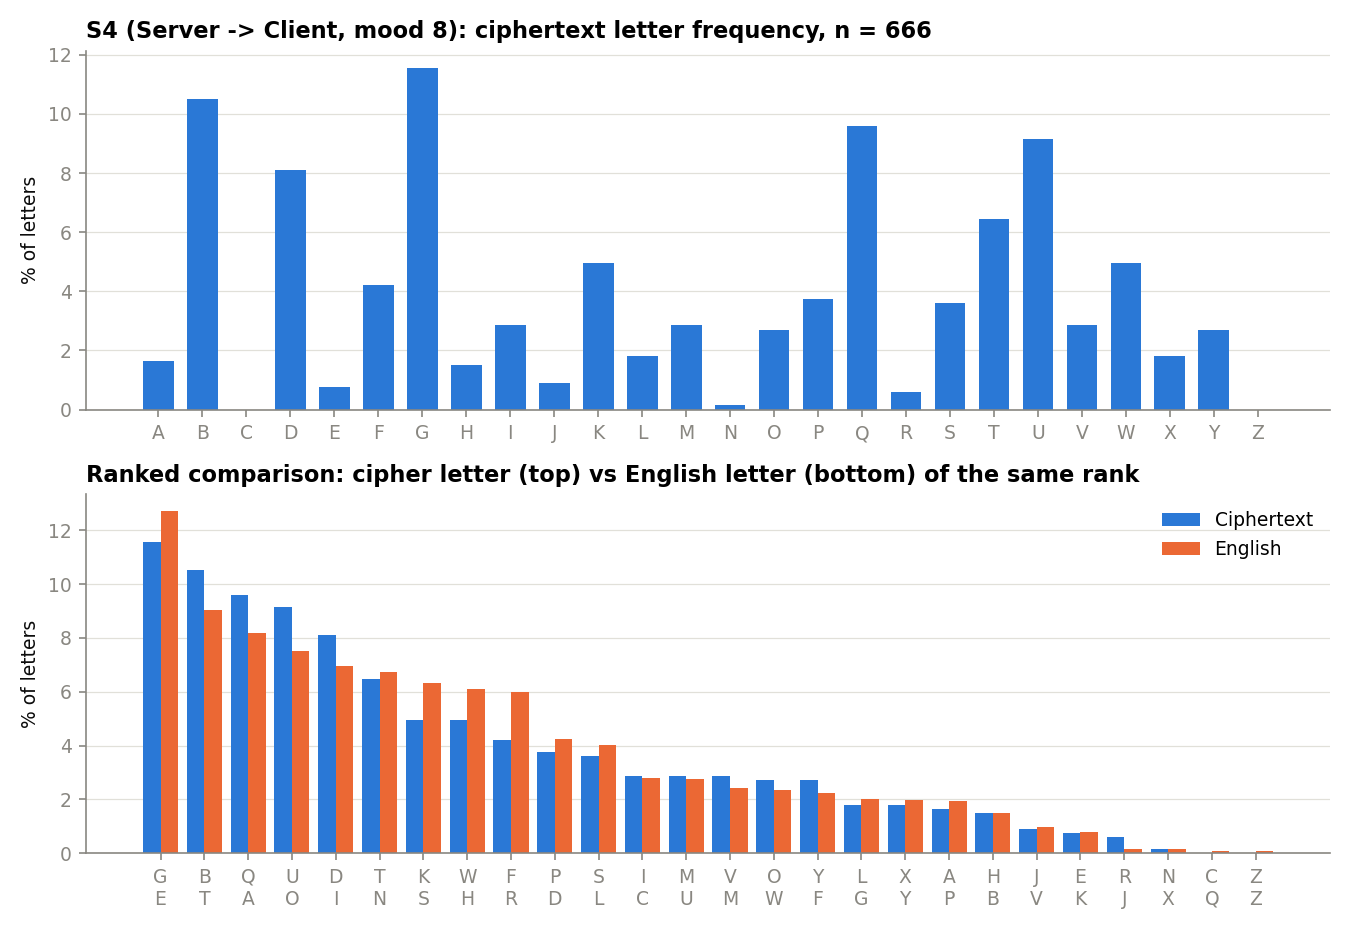
\includegraphics[width=0.8\linewidth]{freq_S4.png}\caption{S4 (mood 8).}\end{figure}
\freqtable{S4}{8}{666}
\clearpage
\begin{figure}[H]\centering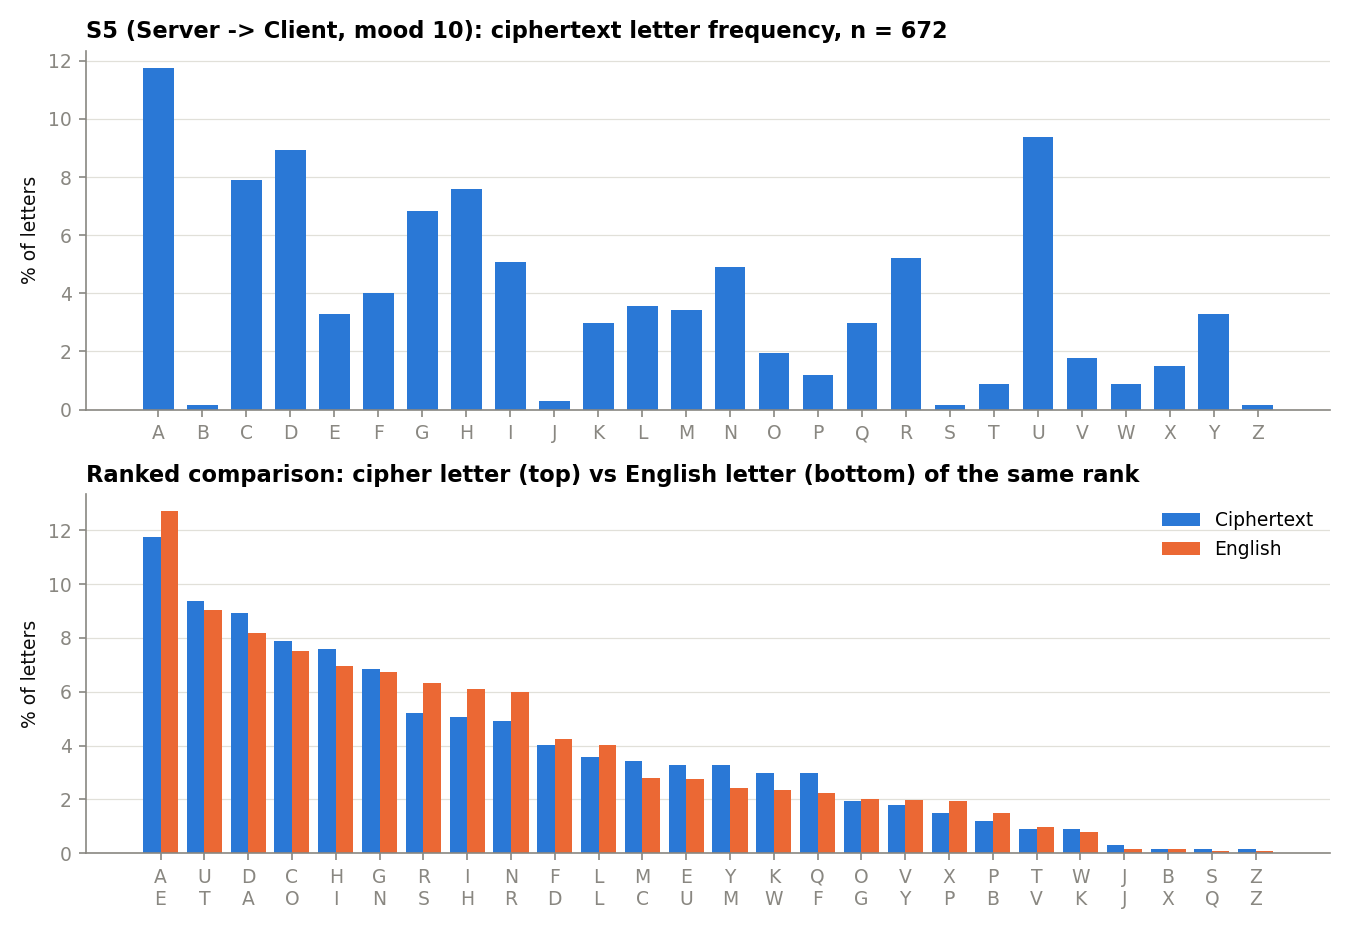
\includegraphics[width=0.8\linewidth]{freq_S5.png}\caption{S5 (mood 10).}\end{figure}
\freqtable{S5}{10}{672}
\clearpage

\subsection*{\csdir{} charts}
\begin{figure}[H]\centering
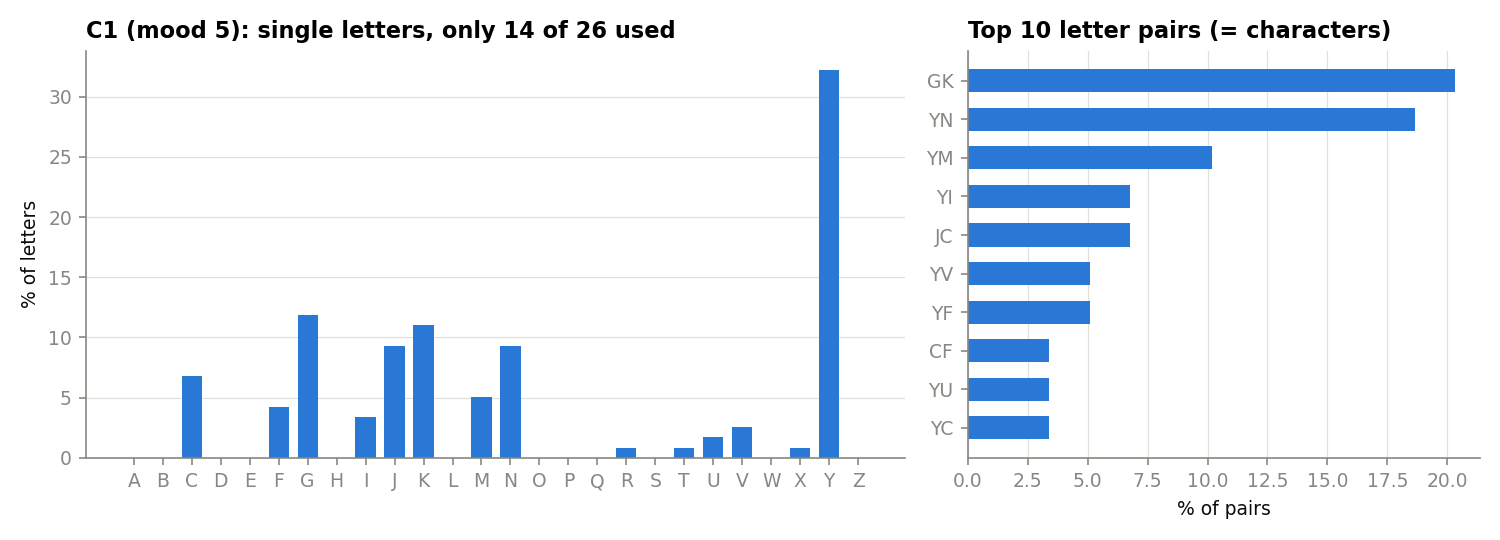
\includegraphics[width=0.9\linewidth]{freq_C1.png}\\[0.3em]
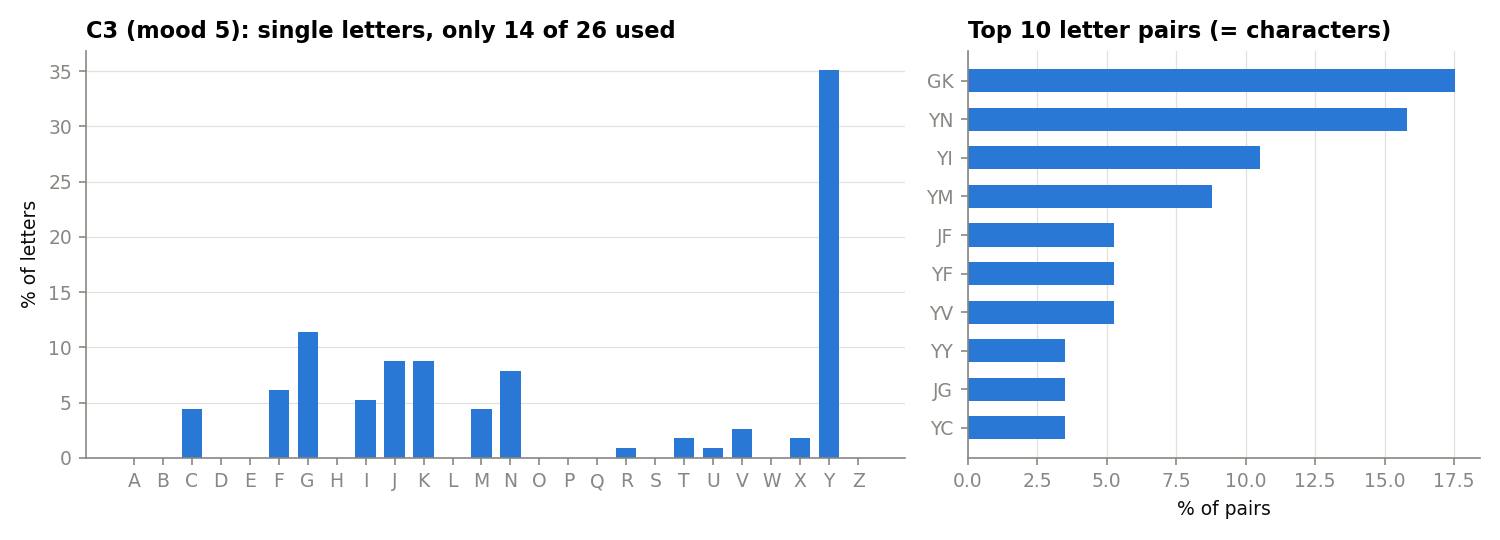
\includegraphics[width=0.9\linewidth]{freq_C3.png}
\caption{C1 and C3 (mood 5).}
\end{figure}
\begin{figure}[H]\centering
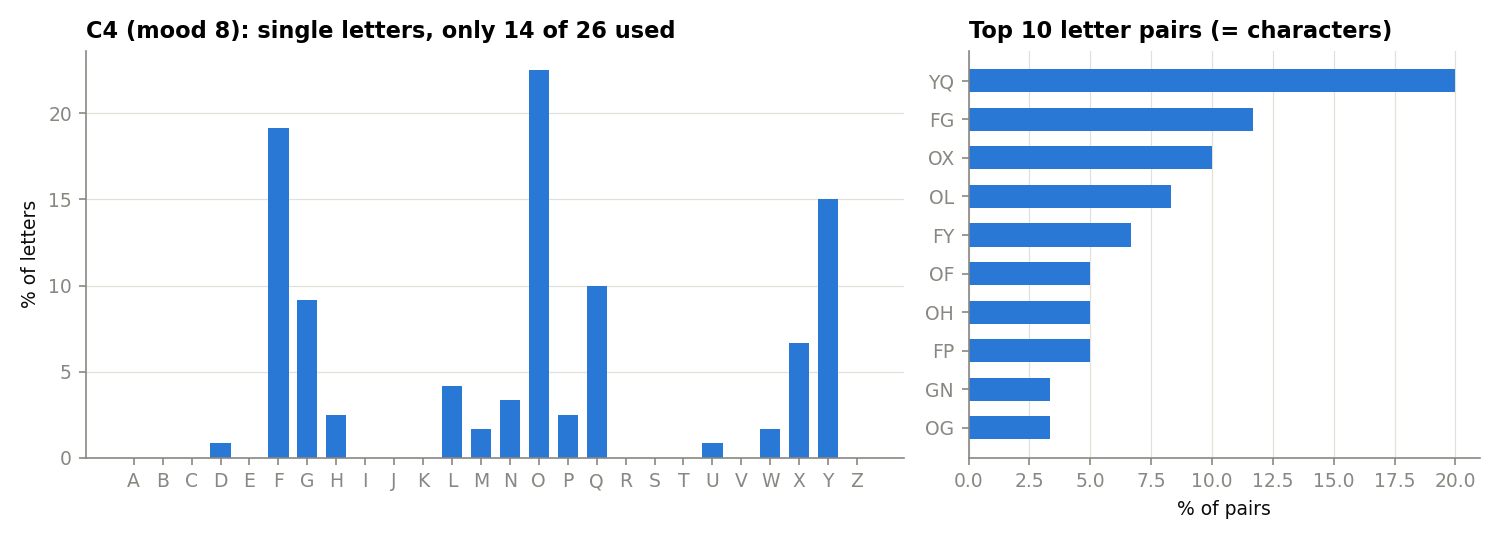
\includegraphics[width=0.9\linewidth]{freq_C4.png}\\[0.3em]
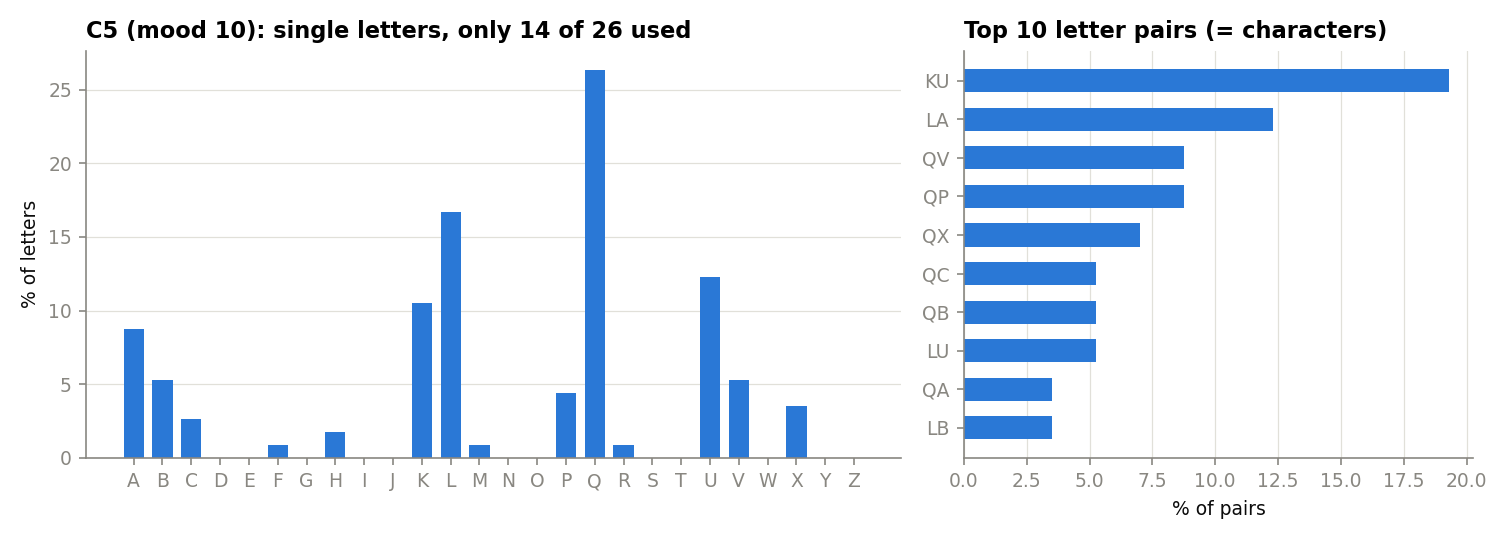
\includegraphics[width=0.9\linewidth]{freq_C5.png}
\caption{C4 (mood 8) and C5 (mood 10).}
\end{figure}

\end{document}
